\documentclass[a4paper, 12pt]{article}
\usepackage[margin=2.5cm]{geometry}
%\usepackage{geometry}[2cm,2cm,2cm,2cm]
\usepackage[utf8]{inputenc}
\usepackage[nosumlimits]{amsmath}
\usepackage{amssymb,stmaryrd,amsthm,MnSymbol}
\usepackage{amsfonts,amssymb,amsopn}
\usepackage{hyperref}
\usepackage{color}
\usepackage{graphicx}
\usepackage{natbib}
\bibliographystyle{elsarticle-harv}
\usepackage{multirow}


%opening
\title{Fully implicit timestepping methods for the rotating shallow water equations}
\author{Werner Bauer\footnote{University of Surrey, UK (w.bauer@surrey.ac.uk), ORCID: \url{https://orcid.org/0000-0002-5040-4287}} \ and
Colin J. Cotter\footnote{Imperial College London, UK, ORCID: \url{https://orcid.org/0000-0001-7962-8324}}}


\newcommand{\todo}[1]{\vspace{5 mm}\par \noindent
	\framebox{\begin{minipage}[c]{0.95 \textwidth}
			\tt #1 \end{minipage}}\vspace{5 mm}\par}
\newcommand{\checkit}[1]{{\color{red}#1}}
\newcommand{\werner}[1]{{\color{magenta}WB says: #1}}
\newcommand{\colin}[1]{{\color{blue}CC says: #1}}
\newcommand{\incl}[1]{{\color{red}#1}}



\DeclareMathOperator{\sat}{sat}
\newcommand{\DD}[2]{\frac{D #1}{D #2}}
\newcommand{\V}{\mathbf{V}}
\newcommand{\U}{\mathbf{U}}
\newcommand{\W}{\mathbf{W}}
\newcommand{\M}{\mathrm{M}}
\newcommand{\R}{\mathrm{R}}
\newcommand{\La}{\mathrm{L}}
\newcommand{\Fu}{\mathbf{F}}


% \newcommand{\D}{\mathbf{D}}
\newcommand{\N}{\mathbf{N}}
\newcommand{\tN}{\tilde{N}}
\newcommand{\tk}{\tilde{k}}
\newcommand{\opL}{\mathcal{L}}
\newcommand{\opN}{\mathcal{N}}



\def\MM#1{\boldsymbol{#1}}
\newcommand{\pp}[2]{\frac{\partial #1}{\partial #2}}
%\newcommand{\dede}[2]{\frac{\delta #1}{\delta #2}}
\newcommand{\dd}[2]{\frac{\diff#1}{\diff#2}}
\newcommand{\dt}[1]{\diff\!#1}
\def\MM#1{\boldsymbol{#1}}
\DeclareMathOperator{\diff}{d}
\DeclareMathOperator{\gat}{\diff\!}
\DeclareMathOperator{\Tr}{Tr}
\DeclareMathOperator{\uu}{\MM{u}^\delta}
\DeclareMathOperator{\F}{\MM{F}^\delta}
\DeclareMathOperator{\D}{D^\delta}
\DeclareMathOperator{\q}{q^\delta}
\DeclareMathOperator{\Z}{Z^\delta}
\DeclareMathOperator{\qr}{\mathring{q}^\delta}
\DeclareMathOperator{\DIV}{DIV}

\newcommand{\jump}[1]{[\![#1]\!]}


\begin{document}

\maketitle

\begin{abstract}
Fully implicit timestepping methods have several potential advantages for atmosphere/ocean simulation. First, being unconditionally stable, they degrade more gracefully as the Courant number increases, typically requiring more solver iterations rather than suddenly blowing up. Second, particular choices of implicit timestepping methods can extend energy conservation properties of spatial discretisations to the fully discrete method. Third, these methods avoid issues related to splitting errors that can occur in some situations, and avoid the complexities of splitting methods.

Fully implicit timestepping methods have had limited application in
geophysical fluid dynamics due to challenges of finding suitable
iterative solvers, since the coupled treatment of advection prevents
the standard elimination techniques. However, overlapping Additive
Schwarz methods, provide a robust, scalable iterative approach for
solving the monolithic coupled system for all fields and Runge-Kutta
stages.

In this study we investigate this approach applied to the rotating
shallow water equations, facilitated by the Irksome package which
provides automated code generation for implicit Runge-Kutta
methods. We compare various schemes in terms of accuracy and
efficiency using an implicit/explicit splitting method, namely the
ARK2 scheme of Giraldo et al (2013), as a benchmark. This provides an
initial look at whether implicit Runge-Kutta methods can be viable for
atmosphere and ocean simulation.
\end{abstract}

\section{Introduction}


\section{Description of methods}
\subsection{Spatial discretisation}
In this article we consider implicit time discretisations for the
rotating shallow water equations on the sphere, which we write
here in vector-invariant form as
\begin{align}
  u_t + \left(\nabla\cdot u^\perp + f\right)u^\perp
  + \nabla\left(\frac{|u|^2}{2} + g(D-b)\right) & = 0, \\
  D_t + \nabla\cdot(uD) & = 0,
\end{align}
where $u$ is the velocity (tangential to the sphere), $\nabla$ is the
gradient projected into the tangent plane on the sphere, $v^\perp =
k\times v$ for vector fields $v$, $k$ is the unit outward pointing
normal to the sphere, $f=2\Omega \sin(\phi)$ is the Coriolis parameter
with $\Omega$ the rotation rate of the Earth (2$\pi$/(sidereal day))
and latitude $\phi$, $g$ is the acceleration due to gravity, $b$ is
the topography field, and $D$ is the depth of the layer.

In this investigation we use a compatible finite element
discretisation of these equations. We do not expect that the precise
details are important for our conclusions, which are hopefully
translatable to other discretisation approaches. However, to
efficiently describe our iterative solver approach a precise
description is useful. We select $V$ as the degree $p+1$ BDM finite
element space on triangles, and $Q$ as the degree $p$ discontinuous
Lagrange finite element space, here defined on an icosahedral grid
$\mathcal{X}$ formed by recursively refining an icosahedron and then projecting
vertices radially out to the sphere. Then we seek $(u,D)\in V\times Q$
such that
\begin{align}
  \label{eq:ut}
  \langle w, u_t \rangle + a(u,D;w) 
   & = 0,
  \quad \forall w \in V, \\
  \label{eq:Dt}
  \langle \phi, D_t \rangle
+ c(u,D; \phi) & =
 0, \quad \forall \phi \in Q,
\end{align}
where
\begin{align}
   a(u,D;w) 
&=
  \langle w, fu^\perp \rangle 
  - \langle \nabla_h^\perp (w\cdot u^\perp), u \rangle
  + \llangle \jump{(w\cdot u^\perp) n^\perp}, \tilde{u} \rrangle  - \left\langle \nabla\cdot w, \frac{|u|^2}{2} + g(D+b) \right\rangle, \\
  c(u,D; \phi) &=
  - \langle \nabla_h \phi, uD \rangle
  + \llangle \jump{\phi n\cdot u}, \tilde{D} \rrangle,
\end{align}
and where $\langle \cdot , \cdot \rangle$ is the usual $L^2$ inner
product defined for scalar or vector fields integrating over the
domain $\mathcal{X}$, $\llangle\cdot,\cdot \rrangle$ is the $L^2$
inner product integrating over the set $\Gamma$ of mesh facets,
$\nabla_h$ is the ``broken'' cellwise gradient, $\tilde{u}$ and
$\tilde{D}$ are the values of $D$ of $u$ evaluated on the upwind side
of a facet (the side with $u\cdot n<0$), $n$ is the unit normal (here,
bivalued so that on each side of the facet $n$ is oriented to point
into the other side), and $\jump{\psi}$ indicates the sum of the
values of $\psi$ over both sides of the facet. For more details, and a
derivation of the finite element spaces and this finite element
approximation, see \cite{gibson2019compatible}. In this work we used
$p=1$.

\subsection{Implicit Runge Kutta time discretisation}

\colin{Define the big space and use big space variables in R}

Runge-Kutta methods advance the solution $U$ from one step $U^n$ to
the next $U^{n+1}$ by computing $s$ stages $(k_1,\ldots,k_s)$ and then
updating the solution according to
\begin{equation}
  U^{n+1} = U^n + \Delta t\sum_{i=1}^s b_i k_i,
\end{equation}
where $b=(b_1,\ldots, b_s)$ are coefficients specific to the
particular chosen Runge-Kutta method. Our spatially discrete rotating
shallow water system (\ref{eq:ut}-\ref{eq:Dt}) is a ``mixed'' coupled
system for two variables, so we write $U=(u,D)\in V\times Q$, and $k_i
= (k_{u,i},k_{D,i})\in V\times Q$ for $i=1,\ldots,s$. Further,
implicit Runge-Kutta methods couple all of these stages together, so it
is useful to define a single variable for all of the stage components,
\[
k = (k_{u,1},k_{D,1},\ldots,k_{u,s},k_{D,s}) \in
\prod_{i=1}^s V\times Q := W.
\]
Implicit Runge-Kutta methods for (\ref{eq:ut}-\ref{eq:Dt}) then 
seek $k\in W$ such that
\begin{align}
    \label{eq:u stages}
    R_{u,i}[k;w] := \langle w, k_{u,i} \rangle + \Delta t a\left(
    u^n_i,D^n_i;w\right)
  & = 0,  
  \quad \forall w \in V,\mbox{ for }i=1,\ldots,s, \\
  \label{eq:D stages}
  R_{D,i}[k;\phi] := \langle \phi, k_{D,i} \rangle + \Delta tc\left(u^n_i,D^n_i; \phi\right)
  & = 0, \quad \forall \phi \in Q, \mbox{ for }i=1,\ldots,s,\\
  u^n_i = u^n + \Delta t\sum_{j=1}^sA_{ij}k_{u,j}, & \mbox{ for }i=1,\ldots,s,\\
  D^n_i = D^n + \Delta t\sum_{j=1}^sA_{ij}k_{D,j}, & \mbox{ for }i=1,\ldots,s,
\end{align}
where $A_{ij}$ are the matrix coefficients from the Butcher
tableau for the chosen Runge-Kutta scheme. This defines a coupled
system for all of the stages in general. After solving
(\ref{eq:u stages}-\ref{eq:D stages}) for the stages, the solution
at the next timestep is obtained from
\begin{equation}
  u^{n+1} = u^n + \Delta t\sum_{i=1}^sb_i k_{u,i},\quad
  D^{n+1} = D^n + \Delta t\sum_{i=1}^sb_i k_{D,i},
\end{equation}
where $b_i$ are also obtained from the Butcher tableau. In this work
we consider collocation Runge-Kutta methods, in particular the
Gauss-Legendre methods that extend the implicit midpoint rule to
higher orders, and the Radau IIA methods that extend the backward Euler
method to higher orders. The Gauss-Legendre methods are energy
preserving for wave equations but slow down high frequency
oscillations, whilst the Radau IIA methods damp high frequency
oscillations.  See \citet{wanner1996solving} for a comprehensive
derivation and analysis of these methods, along with their Butcher
tableau. Note here that our system has no explicit time dependence
which would otherwise need to be incorporated into (\ref{eq:u
  stages}-\ref{eq:D stages}) in the usual way.

We solve the sparse nonlinear system (\ref{eq:u stages}-\ref{eq:D
  stages}) using Newton iteration. Given an initial guess $k\in W$ for
the stages, a Newton iteration requires solving the coupled linear
Jacobian system for corrections
\[
k' = (k'_{u,1},k'_{D,1},\ldots, k'_{u,s},k'_{D,s}) \in W,
\]
such that
\begin{align}
  \nonumber
    \langle w, k'_{u,i} \rangle +
   \Delta t \sum_{j=1}^sA_{ij}\gat a\left(u^n_i,D^n_i;(k'_{u,j}, k'_{D,j}),
   w\right) &=  -R_{u,i}[k;w], \\
   \label{eq:u J}
   & \qquad\qquad    \forall w \in V,\mbox{ for }i=1,\ldots,s, \\
   \nonumber
  \langle \phi, k'_{D,i} \rangle
  + \Delta t\sum_{j=1}^sA_{ij}\gat c\left(u^n_i,D^n_i;(k'_{u,j}, k'_{D,j}),
  \phi\right)  &= -R_{D,i}[k;\phi], \\
  & \qquad \qquad \forall \phi \in Q,\mbox{ for }i=1,\ldots,s.
    \label{eq:D J}
\end{align}
Here, $\gat a$ and $\gat b$ are the Gateaux
derivatives of $a$ and $c$ defined by
\begin{align}
  \gat a(u,D;(v,\phi),w) & = \lim_{\epsilon\to 0}
  \frac{1}{\epsilon}(a(u+\epsilon v,D+\epsilon \phi; w)
  - a(u,D;w)),  \, \forall u,v,w \in V, \, D,\phi \in Q, \\
  \gat c(u,D;(v,\phi),\psi) & = \lim_{\epsilon\to 0}
  \frac{1}{\epsilon}(c(u+\epsilon v,D+\epsilon \phi; \psi)
  - c(u,D;\psi)), \, \forall u,v \in V,\, D,\phi,\psi \in Q,
\end{align}
taking the convention that the upwind switches have derivative
zero\footnote{This treatment means that we are in effect using a
quasi-Newton method; using a semi-smooth Newton method might be
more elegant, but we do not observe any issues with our approach.}
when $u\cdot n=0$.

The solution is then updated according to
\begin{equation}
  k_{u,i}\mapsto k_{u,i} + k'_{u,i}, \quad
  k_{D,i}\mapsto k_{D,i} + k'_{D,i},
\end{equation}
and the iteration is repeated until the residuals in (\ref{eq:u
  stages}-\ref{eq:D stages}) are sufficiently small (according to an
appropriately chosen termination criteria).  The assembly of these
nonlinear and linear systems can be performed in the usual way by
looping (in parallel) over cells and constructing the appropriate
contributions upon substituting $w$ and $\phi$ for each basis function
from standard sparse finite element bases for $V\times Q$. It remains
to find a scalable way to solve (\ref{eq:u J}-\ref{eq:D J}).

We observe that the stage components of the iterative corrections $k'$
are coupled in (\ref{eq:u J}-\ref{eq:D J}) both between $u$ and $D$
components for the same stage $i$ (where the coupling is global but
sparse), as well as between all of the stages from $i=1$ to $s$. This
presents challenges for the solver. In this work, we solve (\ref{eq:u
  J}-\ref{eq:D J}) using a monolithic approach, meaning that we apply
a preconditioned Krylov solver to the full set of basis coefficients
for the iterative corrections $w=\{(k'_{u,i}, k'_{D,i})\}_{i=1}^s$,
treated as a single vector. In our experiments we used FGMRES (the
flexible generalised minimum residual method \citep{saad1993flexible})
for the chosen Krylov method, because we used GMRES (the generalised
minimum residual method \citep{saad1986gmres}) in some inner
iterations in the preconditioner, which we shall describe next.

\colin{FGMRES and GMRES in MG citations}

\begin{figure}
  \center
  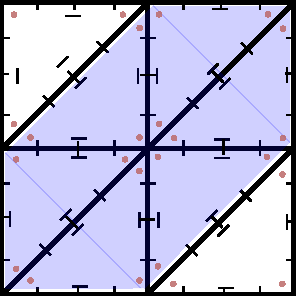
\includegraphics[width=5cm]{Images/patch}
  \caption{\label{fig:patch} A diagram showing the ``vertex
    star'' patch associated with the vertex at the middle of the
    diagram. Dots indicate $D$ degrees of freedom and thin lines
    indicate $u$ degrees of freedom. Of the latter, lines crossing
    cell edges indicate normal components of $u$, which are continuous
    across cell edges for our choice of finite element space.  Lines
    parallel to cell edges indicate tangential components of $u$,
    which are discontinuous across cell edges.  The shaded region
    indicates the patch.  All degrees of freedom outside the shaded
    region (including normal but not tangential components on the
    patch boundary).
  }
 \end{figure}

As a preconditioner, we used geometric multigrid with a sequence of
nested meshes of the spherical domain,\footnote{In fact our meshes are
not strictly nested, because our cells are flat triangles (higher
order polynomial representations are also possible). Starting from the
coarsest icosahedral mesh, each triangle is refined by replacing it
with four smaller triangles, created by adding vertices at the
midpoint of each edge. The new vertices are then moved to the surface
of the sphere being approximated. Transfer operators are defined by
moving the extra vertices of the finer mesh to the edges of the coarse
mesh before prolongation/restriction.} with prolongation operators
consisting of the inclusion operator, \emph{i.e.} reinterpretation of
the same function in the larger space on the finer mesh; restriction
is taken as \checkit{the $L_2$ the dual???} of prolongation.\werner{sentence?}

For smoothers on each level, we used an additive Schwarz method that
is built using overlapping subspaces $W_l=V_l\times Q_l \subset W =
\prod_{i=1}^s\left(V \times Q\right)$, $l=1,\ldots,N_l$, where $W$ is
the mixed finite element space comprising all of the stages.
In this work we define the subspaces $W_l$ using ``vertex
star patches''.  Here, there is one subspace for each of the $M$
vertices in the mesh.  The subspace for a vertex $z_l$ is defined by
taking the set $S_l$ of cells surrounding $z_l$. $W_l$ is the subspace
of $W$ consisting of functions that are equal to zero when restricted
to any cell not in $S_l$. For our choice of spaces, this entails
zeroing any degrees of freedom on the boundary of $S_l$ and beyond
(See Figure \ref{fig:patch}). In the multigrid algorithm, the goal of
the smoother is to approximately solve a problem of the form
(\ref{eq:u J}-\ref{eq:D J}) but with $R_{u,i}$ and $R_{D,i}$ replaced
by residuals provided from the next finest grid.  For the additive
Schwarz method, we solve (\ref{eq:u J}-\ref{eq:D J}) with solutions
$w_l$ and test functions restricted to $W_l$, using a direct
solve. These ``patch problems'' can be solved independently and in
parallel using a dense direct solver.  Then, the additive Schwarz
approximate solutions are obtained as $\sum_{l=1}^{N_l}w_l$ (here
$w_l$ is interpreted as a function in $W$ by inclusion $W_l\subset
W$).

The reason for choosing vertex star patches is that they deal well
with the oscillatory wave coupling in the linear system. When this
form of multigrid is applied to the rotating shallow water equations
linearised about a state of rest (referred to as the linear rotating
shallow water equations), we observe mesh- and $\Delta t$-robust
convergence rates. This is believed to be related to the efficacy of
vertex star patches for Hdiv problems \citep{arnold2000multigrid} but
there is no analysis for monolithic multigrid applied to mixed
elliptic problems at present \citep{sm}. The reason for choosing patches
that couple between all stages is that we aim to obtain robust
convergence in the number of Runge-Kutta stages, as analysed in
\citep{kirby2024convergence}.

To avoid having to tune scaling parameters whose optimal values might
depend on the system state, our smoothers consist of two iterations of
GMRES preconditioned by the additive Schwarz method above. This has
the effect of selecting the scaling parameter adaptively.  This
necessitates the use of a flexible Krylov method (FGMRES, in our
case), since the use of GMRES means that the smoother is residual
dependent and hence is not a stationary iterative method (which is a
requirement for standard Krylov methods such as GMRES).

In our multigrid setup, we also used the above smoothing approach for
the correction on the coarsest grid. This avoids having to use a
parallel direct solve. We experimented with a direct solve on the coarse
grid but found that it did not alter the overall convergence of the
solver strategy.

As will become apparent from the results, we do not observe perfect
multigrid behaviour in that the number of iterations is not robust in
$\Delta t$: more iterations are required at larger $\Delta t$ due to
the presence of the advective terms.  For this type of problem, it is
also typical to scale $\Delta t$ to keep the advective Courant number
($U\Delta t/\Delta x$ where $U$ is a typical velocity scale and
$\Delta x$ is a typical cell diameter) constant as the mesh is
refined, so we can hope for mesh independent Krylov iteration counts
under this refinement scaling without multigrid. However, we found
that using the multigrid produced faster wallclock times.

As a final optimisation, we used the Eisenstat-Walker (version 2)
inexact Newton approach \citep{eisenstat1996choosing} which adaptively
controls the number of Krylov iterations for the Jacobian system
during the Newton algorithm, since it is not useful to solve the
Jacobian system accurately when the nonlinear solution is only going
to be iteratively updated again anyway. This reduces the overall
number of Krylov iterations per timestep, and hence reduces the overall
number of multigrid cycles which dominate the cost of the method.

In this work we implemented this approach using Irksome
\citep{farrell2021irksome,kirby2024extending}, a Python library that
wraps time discretisations on top of finite element spatial
discretisations implemented using Firedrake
\citep{FiredrakeUserManual}, an automated system for the solution of
partial differential equatoins using the finite element method.  This
combination in turn makes significant use of PETSc
\citep{dalcin2011parallel,balay2019petsc}. In particular, PETSc's and
Firedrake's PCPatch implementation of additive Schwarz methods is used
\citep{farrell2021pcpatch}.  Amongst the benefits of this approach to
implementation, Firedrake uses automated differentiation provided by
the Unified Form Language (UFL) \citep{alnaes2012ufl} to obtain the
formulae for (\ref{eq:u J}-\ref{eq:D J}) from which code assembling
the matrix-vector action and the patch linear systems is automatically
generated.

\subsection{Implicit-explicit time discretisation}

We compared our implicit Runge-Kutta approach with an
implicit-explicit (IMEX) time discretisation. This serves as a
benchmark in terms of timing since IMEX methods are well known in the
community developing numerical methods for geophysical fluid dynamics.
We choose one specific second-order IMEX scheme, the ARK2 scheme
of \citet{giraldo2013implicit}, which they demonstrated to be optimal
for geophysical fluid problems amongst second order IMEX schemes and has
been widely adopted in the field.

To produce an IMEX scheme, we rewrite our spatial discretisation
(\ref{eq:ut}-\ref{eq:Dt}) in the form
\begin{align}
  \label{eq:ut IMEX}
  \langle w, u_t \rangle + a_L(u,D;w) 
  + a_N(u,D;w) 
   & = 0,
  \quad \forall w \in V, \\
  \label{eq:Dt IMEX}
  \langle \phi, D_t \rangle
+ c_L(u,D; \phi) + c_N(u,D; \phi)  & =
 0, \quad \forall \phi \in Q,
\end{align}
where $a_L$, $a_N$ are the linear and nonlinear operators for $u$,
and $c_L$, $c_N$ are the linear and nonlinear operators for $D$,
defined by
\begin{align}
  a_L(u,D;w) & = \langle w, fu^\perp \rangle - \langle \nabla\cdot w,
  gD \rangle, \\
   a_N(u,D;w) 
&=
  - \langle \nabla_h^\perp (w\cdot u^\perp), u \rangle
  + \llangle \jump{(w\cdot u^\perp) n^\perp}, \tilde{u} \rrangle  - \left\langle \nabla\cdot w, \frac{|u|^2}{2} + gb \right\rangle, \\
  c_L(u,D;\phi) & = \langle \phi, H\nabla\cdot u\rangle, \\
  c(u,D; \phi) &=
  - \langle \nabla_h \phi, uD \rangle
  - \langle \phi, H\nabla\cdot u\rangle
  + \llangle \jump{\phi n\cdot u}, \tilde{D} \rrangle.
\end{align}
\colin{explain $L$ is linearisation about state of rest; slow-fast}

In our setting, IMEX schemes take the form,
\begin{align}
    \nonumber
    \langle w, Y_{u,i}-u^n \rangle + \Delta t \sum_{j=1}^{i-1} A_{ij} a_N\left(
    Y_{u,j}, Y_{D,j}; w\right) & \\
\qquad    + \Delta t \sum_{j=1}^i \tilde{A}_{ij} a_L(Y_{u,j}, Y_{D,j}; w)
    & = 0, \label{eq:u stages IMEX}
  \quad \forall w \in V,\mbox{ for }i=1,\ldots,s, \\
  \nonumber
    \langle \phi, Y_{D,i}-D^n \rangle + \Delta t \sum_{j=1}^{i-1} A_{ij} c_N\left(
    Y_{u,j}, Y_{D,j}; \phi\right) & \\
    + \Delta t \sum_{j=1}^i \tilde{A}_{ij} c_L(Y_{u,j}, Y_{D,j}; w)
    & = 0, \label{eq:D stages IMEX}
      \quad \forall \phi \in Q,\mbox{ for }i=1,\ldots,s,
\end{align}
where $A$ and $\tilde{A}$ are the explicit and implicit IMEX Butcher
matrices respectively. Then, we reconstruct the solution from
\begin{align}
  \langle w, u^{n+1} - u^n\rangle + \Delta t\sum_{i=1}^s b_i
  a_N(Y_{u,j}, Y_{D,j}; w)
  + \Delta t \sum_{i=1}^s \tilde{b}_i
  a_L(Y_{u,j}, Y_{D,j}; w)=0,\, \forall w \in V, \\
    \langle \phi, D^{n+1} - D^n\rangle + \Delta t\sum_{i=1}^s b_i
  c_N(Y_{u,j}, Y_{D,j}; \phi)
  + \Delta t \sum_{i=1}^s \tilde{b}_i
    c_L(Y_{u,j}, Y_{D,j}; \phi)=0,\, \forall \phi \in Q,
\end{align}
where $b$ and $\tilde{b}$ are the corresponding IMEX Butcher
reconstruction vectors. Due to the lower triangular structure
expressed in the sum limits, (\ref{eq:u stages IMEX}-\ref{eq:D stages
  IMEX}) can be solved as single coupled mixed problems for
$(Y_{u,i},Y_{D,i})$ at stage $i$. Further, these problems can be
reduced to a sparse ``modified Helmholtz'' type problem for a single
variable using the hybridisation technique for mixed finite elements
\citep{boffi2013mixed,cockburn2004characterization}; similar sparse
reduction techniques exist for finite volume and discontinuous
Galerkin methods. The resulting sparse system can be solved using a
sparse parallel direct solver, or for larger problems, multigrid
methods. In this work we found that sparse direct solvers were quicker
for the 2D problems under consideration. The implicit IMEX linear
systems are state independent, and so can be assembled and factorised
once, which makes their solution very fast. In contrast, the patch
problems used for the IRK methods depend on the system state, and must
be refactorised for each Jacobian solve.

The ARK2 IMEX scheme is a 3 stage scheme involving two implicit solves
per timestep. It was implemented using Firedrake again, using the
hybridization solver package SLATE \citep{gibson2020slate} for the
implicit linear systems.

\section{Numerical results}


\begin{itemize}
 \item Describe test case Williamson 6
 \item Describe mesh levels somehow!!!
\end{itemize}

Some details of solver options

In this section we test the monolithic solver setup with fully implicit time stepping methods introduced above concerning their performance. We will discuss different orders of accuracy for two realizations, namely the Gauss Legendre method and the Radau 2 method, both fully implicit schemes for various order, i.e. for orders 1,2, and 3 \checkit{ADD CORRECT VALUES.} We compare these methods with the frequently used, very efficient IMEX method ARK2, as introduced in CITE by CITE:Giraldo13.

The aim is to test this for geophysical applications, i.e for atmosphere and ocean simulations. Hence, we select a testcase that allows us to best identify error sources of the time integrator before spacial errors dominate. To this end, we use the Williamson 6 test case where a solid wave is transported around the globe. Simulating it for a relatively short time of 1 day allows us to identify time integrator errors, mitigation inpact of small scale errors triggered by nonlinearies that might dominate the error for longer integrations.

The essential quantities of interest for operational simulations are the total runtime of a simulation and the relative errors the integrators have. As such, we compare exactly those two quantities for various parameter choices for our implicit methods and for the imex schemes. As we will see, accuracy and runtime crucially depend on the selected time step sizes and hence, those are added too to the graphics we present below to have an idea how the selection of step sizes impact on accuracy and runtime for imex and irksome runs.


\begin{figure}[t]\centering
 \begin{tabular}{cc}
 \hspace{-0em}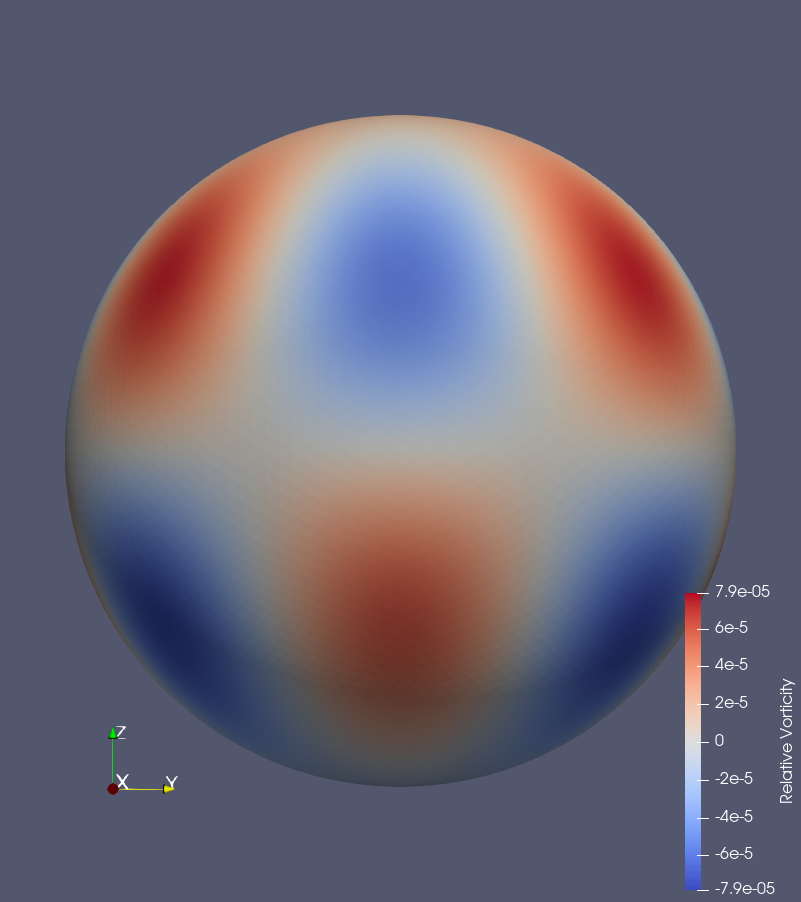
\includegraphics[scale=0.125]{Images/vorticity_0.png} &
 \hspace{-0em}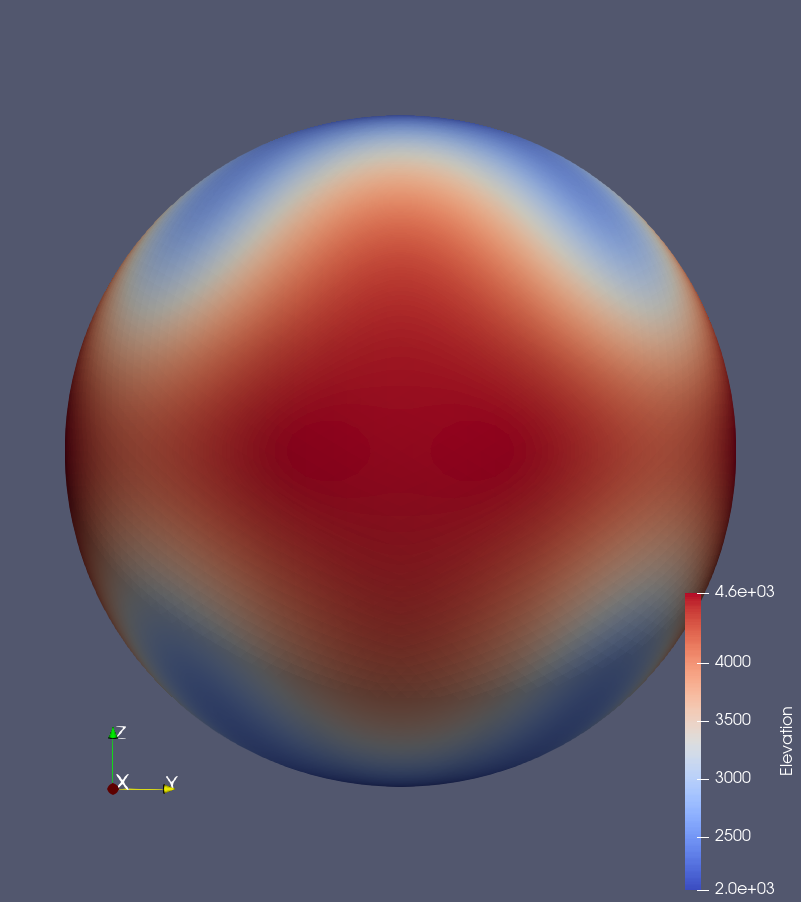
\includegraphics[scale=0.125]{Images/elevation_0.png} \\
 \hspace{-0em}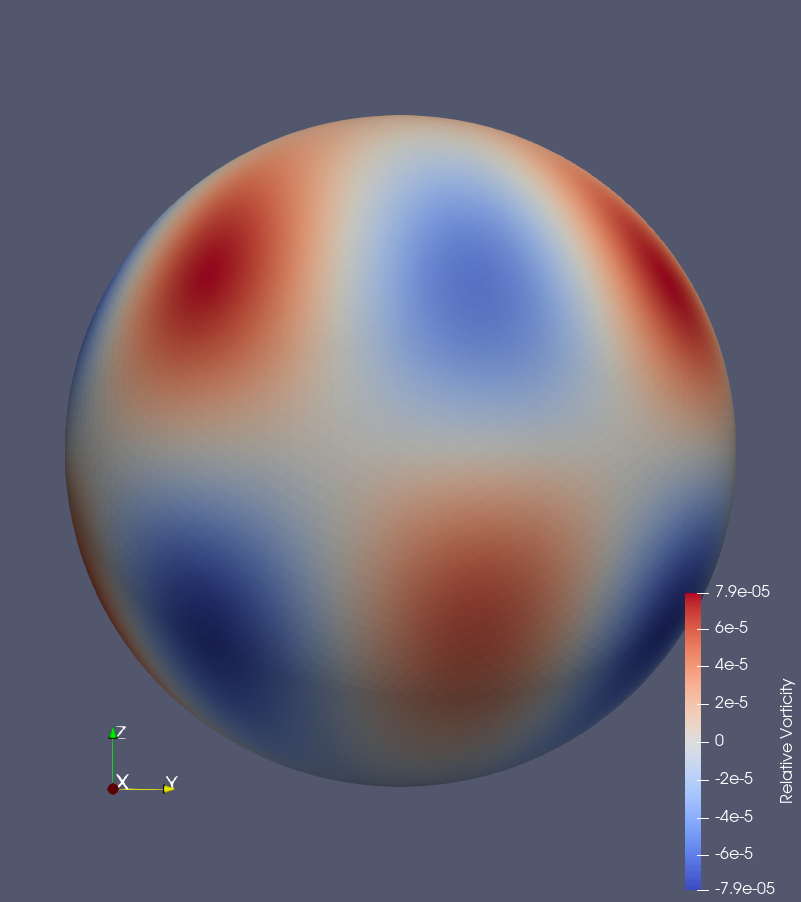
\includegraphics[scale=0.125]{Images/vorticity_24.png} &
 \hspace{-0em}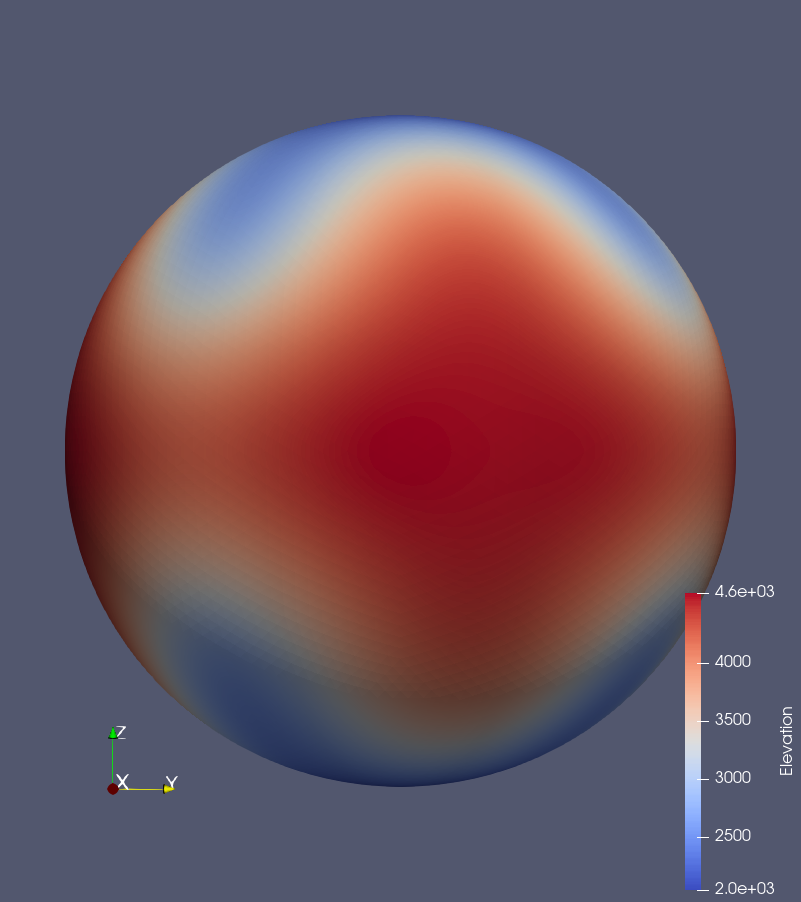
\includegraphics[scale=0.125]{Images/elevation_24.png} \\
 \end{tabular}\vspace{-10pt}
  \caption{Top row: initial vorticity (left column) and depth (right column) fields
  for Williamson test case 6. Bottom row: both fields at day 1. The shown fields are for mesh level 5.
  }
 \label{tc6_fields}
\end{figure}



\subsection{Comparison with Runga-Kutta IMEX schemes}

\newcommand{\ybf}{\mathbf{y}}
\newcommand{\sbf}{\mathbf{s}}
\newcommand{\fbf}{\mathbf{f}}

Before we introduce the test case, let us quickly recall the implicit/explicit
splitting method ARK2 of Giraldo et al (2013) that we use as a benchmark.
To this end, let us consider the following ordinary differential equation (ODE)
\begin{equation}
\frac{d}{dt} \mathbf{y} = \mathbf{s}(\mathbf{y}, t) + \mathbf{f} (\mathbf {y}, t).
\end{equation}
The vectors $\mathbf{y}, \mathbf{s} , \mathbf{f}$ can include various state variables.
The time scale associated with $ \mathbf{s}(\mathbf{y}, t)$ is relatively long
and can be solved explicitly while those associated with $\mathbf {y}$
can be very short so $ \mathbf{f} (\mathbf {y}, t)$ must be solved implicitly.

In general, a Runga-Kutta IMEX scheme is defined by $\nu$ sub-stages (indexed with $j$ and first equation below) and one final stage (second equation below) to advance the time from time level $t^n$ to $t^{n+1}$ with time step size $\Delta t$ such that
$t^{n+1} = t^n + \Delta t$, namely:
\begin{align}
&  \ybf^{(j)}  = \ybf^n + \Delta t \sum_{l=1}^{j-1} \tilde a_{jl} \,  \sbf(\ybf^{(l)}, t^n + \tilde c_{l}\Delta t) + \Delta t \sum_{l=1}^{j} a_{jl} \,  \fbf(\ybf^{(l)}, t^n + c_{l}\Delta t) \, ,  \quad j = 1,...\nu \, , \\
&  \ybf^{n+1}  = \ybf^n + \Delta t \sum_{j=1}^{\nu} \tilde w_{j} \,  \sbf(\ybf^{(j)}, t^n + \tilde c_{j}\Delta t) + \Delta t \sum_{j=1}^{\nu} w_{j} \,  \fbf(\ybf^{(j)}, t^n + c_{j}\Delta t) \, .
\end{align}
The concrete RK-IMEX schemes are then defined by a double Butcher tableau. Here we present the Butcher tableau for the ARK2 (2,3,2) method that we used for our study. That is, for $\nu = 3$, we have, respectively for the explicit (using tilde) and the implicit parts:

%\begin{table}[h]\centering
\begin{tabular}{c|c}
 $\mathbf{\tilde c}$ & $\tilde A$ \\ \hline
    & $\mathbf {\tilde w}^T$
\end{tabular} \ =
\begin{tabular}{c|ccc}
0         &  0             &   0       & 0  \\
$2\gamma$ &  $2\gamma$     &  0        & 0  \\
$1$       & $1 - \alpha$   & $\alpha$  & 0  \\ \hline
          & $\delta$       & $\delta$  & $\gamma$
\end{tabular}  , \qquad
\begin{tabular}{c|c}
 $\mathbf{c}$ & $A$ \\ \hline
    & $\mathbf {w}^T$
\end{tabular} \ =
\begin{tabular}{c|ccc}
0         &  0             &   0       & 0  \\
$2\gamma$ &  $\gamma$     &  $\gamma$        & 0  \\
$1$       & $\delta $   & $\delta$  & $\gamma$  \\ \hline
          & $\delta$       & $\delta$  & $\gamma$
\end{tabular}  , \\
%\end{table}
where $\gamma = 1 - \frac{1}{\sqrt{2}}$, $\alpha = \frac{1}{6} (3 + 2\sqrt{2})$ and
$\delta =  \frac{1}{ 2 \sqrt{2}}$. For $j,l =1,...\nu$, we use the following notation: for explicit part we write
$\mathbf{\tilde c} = \{\tilde c_j\}$,
$\mathbf{\tilde w} = \{\tilde w_j\}$, and
$\tilde A = \{\tilde a_{jl}\}$ where the coefficients must have $\tilde a_{jl} = 0$ for $j \geq l$. For the implicit part, we use
$\mathbf{c} = \{c_j\}$,
$\mathbf{w} = \{w_j\}$, and $A = \{a_{jl}\}$ with $\tilde a_{jl} = 0$ for $j > l$ to obtain a diagonally implicit RK scheme. Depending on the choice of these Butcher tableaus, various RK IMEX schemes can be formulated. For such general formulation and an explicit presentation of the corresponding Butcher tableau, \checkit{see Hillary Weller.}

\todo{
\werner{Stuff from poster: do we need something here?}
We consider the ODE $y'(t) + F(t,y)= 0$ where $y:(0,T] \rightarrow \mathbb{R}^n$ with $y(0) = y_0$
and $F:(0,T]\times \mathbb{R}^n \rightarrow \mathbb{R}^n$.
Given the solution
$y(t^n)\equiv y^n$ and some $t^{n+1} = t^n + \Delta t$, Runga-Kutta (RK) methods approximate $y(t^{n+1})$ by
$y^{n+1} = y^{n} + \Delta t \sum_{i = 1}^{s} b_i k_i,$ where for all $1\leq i \leq s$
 the stages $k_i \in \mathbb{R}^n$ satisfy
\begin{align*}
%  y^{n+1} = y^{n} + \Delta t \sum_{i = 1}^{s} b_i k_i, \
%  \text{where for all $1\leq i \leq n$
%  the stages $k_i \in \mathbb{R}^n$ satisfy} \\
 k_i + F\Big(t + c_i \Delta t, \  y + \Delta t \sum_{j = 1}^{s} A_{ij} k_j \Big) = 0 \
 \text{with $A_{ij}, b_i, c_i$ for $1\leq i,j\leq s$.}
\end{align*}
$A_{ij}, b_i, c_i$ are typically organized in a \emph{Butcher tableau} and determine the order of accuracy.
}
\vspace{0.7cm}


As we will see below, because it is partly explicity, the latter part underlies the CFL criterion, hence the method has a hard time step size restriction. In fact, for our setup we indeed did not achieve stable runs with a time step size larger than about $dt \approx 100s$.

\begin{itemize}
 \item Add solver strategy for IMEX:
 \item EAch of these stages you solve only one hybridized mixed helmholz problem, we store the LU decomposition, it's always the same way equation because the implicit (I) part is the linear wave equation
 \item here the expensive part is forming the LU decomposition, only once, this is why it is hard to beat imex.
\end{itemize}




\subsection{WORK OUT WHAT THE SPACIAL ERROR IS!!!}

\begin{itemize}
 \item velocity field has to be interpolated from one mesh to another, might be worrying, meshes are quite different.
 \item compare 1s l5 vs l6:
 \begin{itemize}
  \item before making comparisons
  \item move back the l6 mesh to l5: i.e. add the coordinate field to that!!!
  \item Colin will help me (during next week)!
  \item Write a paragraph about how this is done!!!
  \item for h it will be sufficient to interpolate from l6 to l5! Go via DG
  \item Let's start first with the h field and then check if we need velocity field!
 \end{itemize}

The results from what we have used so far for the plots!
\begin{itemize}
\item Spacial error in the eta field:  6.720143e-04
\item Spacial error in the vel field:  7.984353e-03
\end{itemize}
We compute the solution for L5 and project it onto the mesh of L6 and then compared this interpolated solutions with the ones directly computed on L6. We compute the relative error by determine the following:
\begin{equation}
err(f, fh) =  \frac{||f_{l6} - f_{l5}||}{||f_{l6}||}
\end{equation}
i.e. relative to the L2 value of $f$ on mesh level L6. Note that usually, $f_{l5}$ has been interpolated
already to the mesh level L6 in order to have a well defined error norm.


\end{itemize}

\newpage





\subsection{Test case description}

We aim to compare the time integrators for applications of geophysical relevance, especially for atmosphere and ocean simulations. Further, we want to compare errors resulting from the time integrators while eliminating as much as possible other error sources such that the difference of the performance of the time integrators gets visible. Therefore, we use the Williamson 6 test case for a simulation time of 1 day. In this test case, a solid wave is transported around the globe. Simulating it for a relatively short time of 1 day allows us to identify time integrator errors, mitigation inpact of small scale errors triggered by nonlinearies that might dominate the error for longer integrations.

The test case description, initialization on parameter values can all be found in the seminar paper of \cite{WILLIAMSON1992211} (Section 6, Rossby-Haurwitz Wave). Figure~\ref{tc6_fields} shows in the top row the initial fields for vorticity (left column) and depth field (right column). The bottom row shows these fields after a simulation time of 1 day. From the figures the solid body rotation of these fields gets obvious.


% The initial conditions reads as follows:
% \begin{itemize}
%  \item $R0 = 6371220$,
%  \item $H = 5960$.
%  \item $\Omega = 7.292e-5$  rotation rate
%  \item $cz$ z-coordinate normal to Earth surface
%  \item $f = 2*\Omega*cz/R0$   Coriolis parameter
%  \item $g = 9.8$   Gravitational constant
%  \item $b$  Topography,
%  \item Sound speed $c = g*H$
% \end{itemize}



\subsection{Simulation results}

We compare the solutions obtained from the studied time integrators with relatively
large time step sizes (i.e. all methods including IMEX use values of $dt >18.5s$) with a reference solutions determined with a very small time step size of $dt=1s$. Because all methods converge with small
$dt$, any of the methods can be used to compute the reference solution: we used the Gauss-Legendre method of order 1 and $dt=1$, for example.

We run each simulation for 1 day and then compute the L2 errors for depth and velocity fields between the coarse time step runs and the reference run for a fixed mesh resolution. For the latter we use a relatively fine mesh resolution of Level 6 (corresponding to approx ???km edge length of the triangulation of the sphere). Besides computing these relative errors, we record for each simulation the total runtime.

Figure~\ref{err_vs_runtime_gl_imex} and Figure~\ref{err_vs_runtime_rd_imex} show the results of this experiment in a concise manner. We used two different implicit Runga-Kutta methods, namely the GaussLegendre method of orders \checkit{1, 3, 5 and the RadauIIA method, or orders 1,2,3}. Points on the curves indicate the total runtime for a chosen method and the obtain accuracy. As both these values depend heavily on the selected time step size, the latter is indicated as numbers (in seconds) on the curves too.


Let's consider first Figure~\ref{err_vs_runtime_gl_imex}, but the discussion is very similar for  Figure~\ref{err_vs_runtime_rd_imex}. We see that with GL, we can go up to a time step size of 14400s. For larger values, it get's more and more difficult for the solver to find an accurate solution, so often the solver does not converge any more if $dt$ is even bigger. Nevertheless, compared to IMEX that is partly explicit and hence underlies the CFL criteria, this time step size is huge. The total runtime for GL1 reduces for such large time step size to less then 100s, however, for a relative error at the order of around 10e-2. Note that both eta and vel have similar orders of error, so we do not distinguish between them in our discussion here and henceforth.

Reducing the time step sizes leads for any of the selected method orders to an increase in accuracy, but with the cost of longer total runtimes. The kinks in the curves for large time step sizes (e.g. for 14400, 10800, 7200) might be related to jumps in the number if iterations required to obtain the desired solver tolerance but for smaller values in $dt$ the indicated relationship between $dt$ and total runtime gets clearer. Smaller $dt$ also leads to more accurate solutions in all cases while methods with higher order are generally more accurate, but because of the increased number of DoF also slower.

Let us next consider the results for the Imex method (red curves in Figure~\ref{err_vs_runtime_gl_imex} and Figure~\ref{err_vs_runtime_rd_imex}). In general we can see that for the chosen second order Imex method (ARK2), the largest possible time step size for the given mesh level L6 is about 100s, restricted through the CFL condition related to the explicit part in the IMEX method. Nevertheless of this restriction, IMEX is a highly efficient scheme giving high performance of about 660s of total runtime with
an accuracy at the order of 10e-5. Also here, reducing $dt$ leads to an increase in accuracy but to the costs of an increase in total runtime.







\begin{figure}[h]\centering
\begin{tabular}{c}
 \hspace{-0.0em}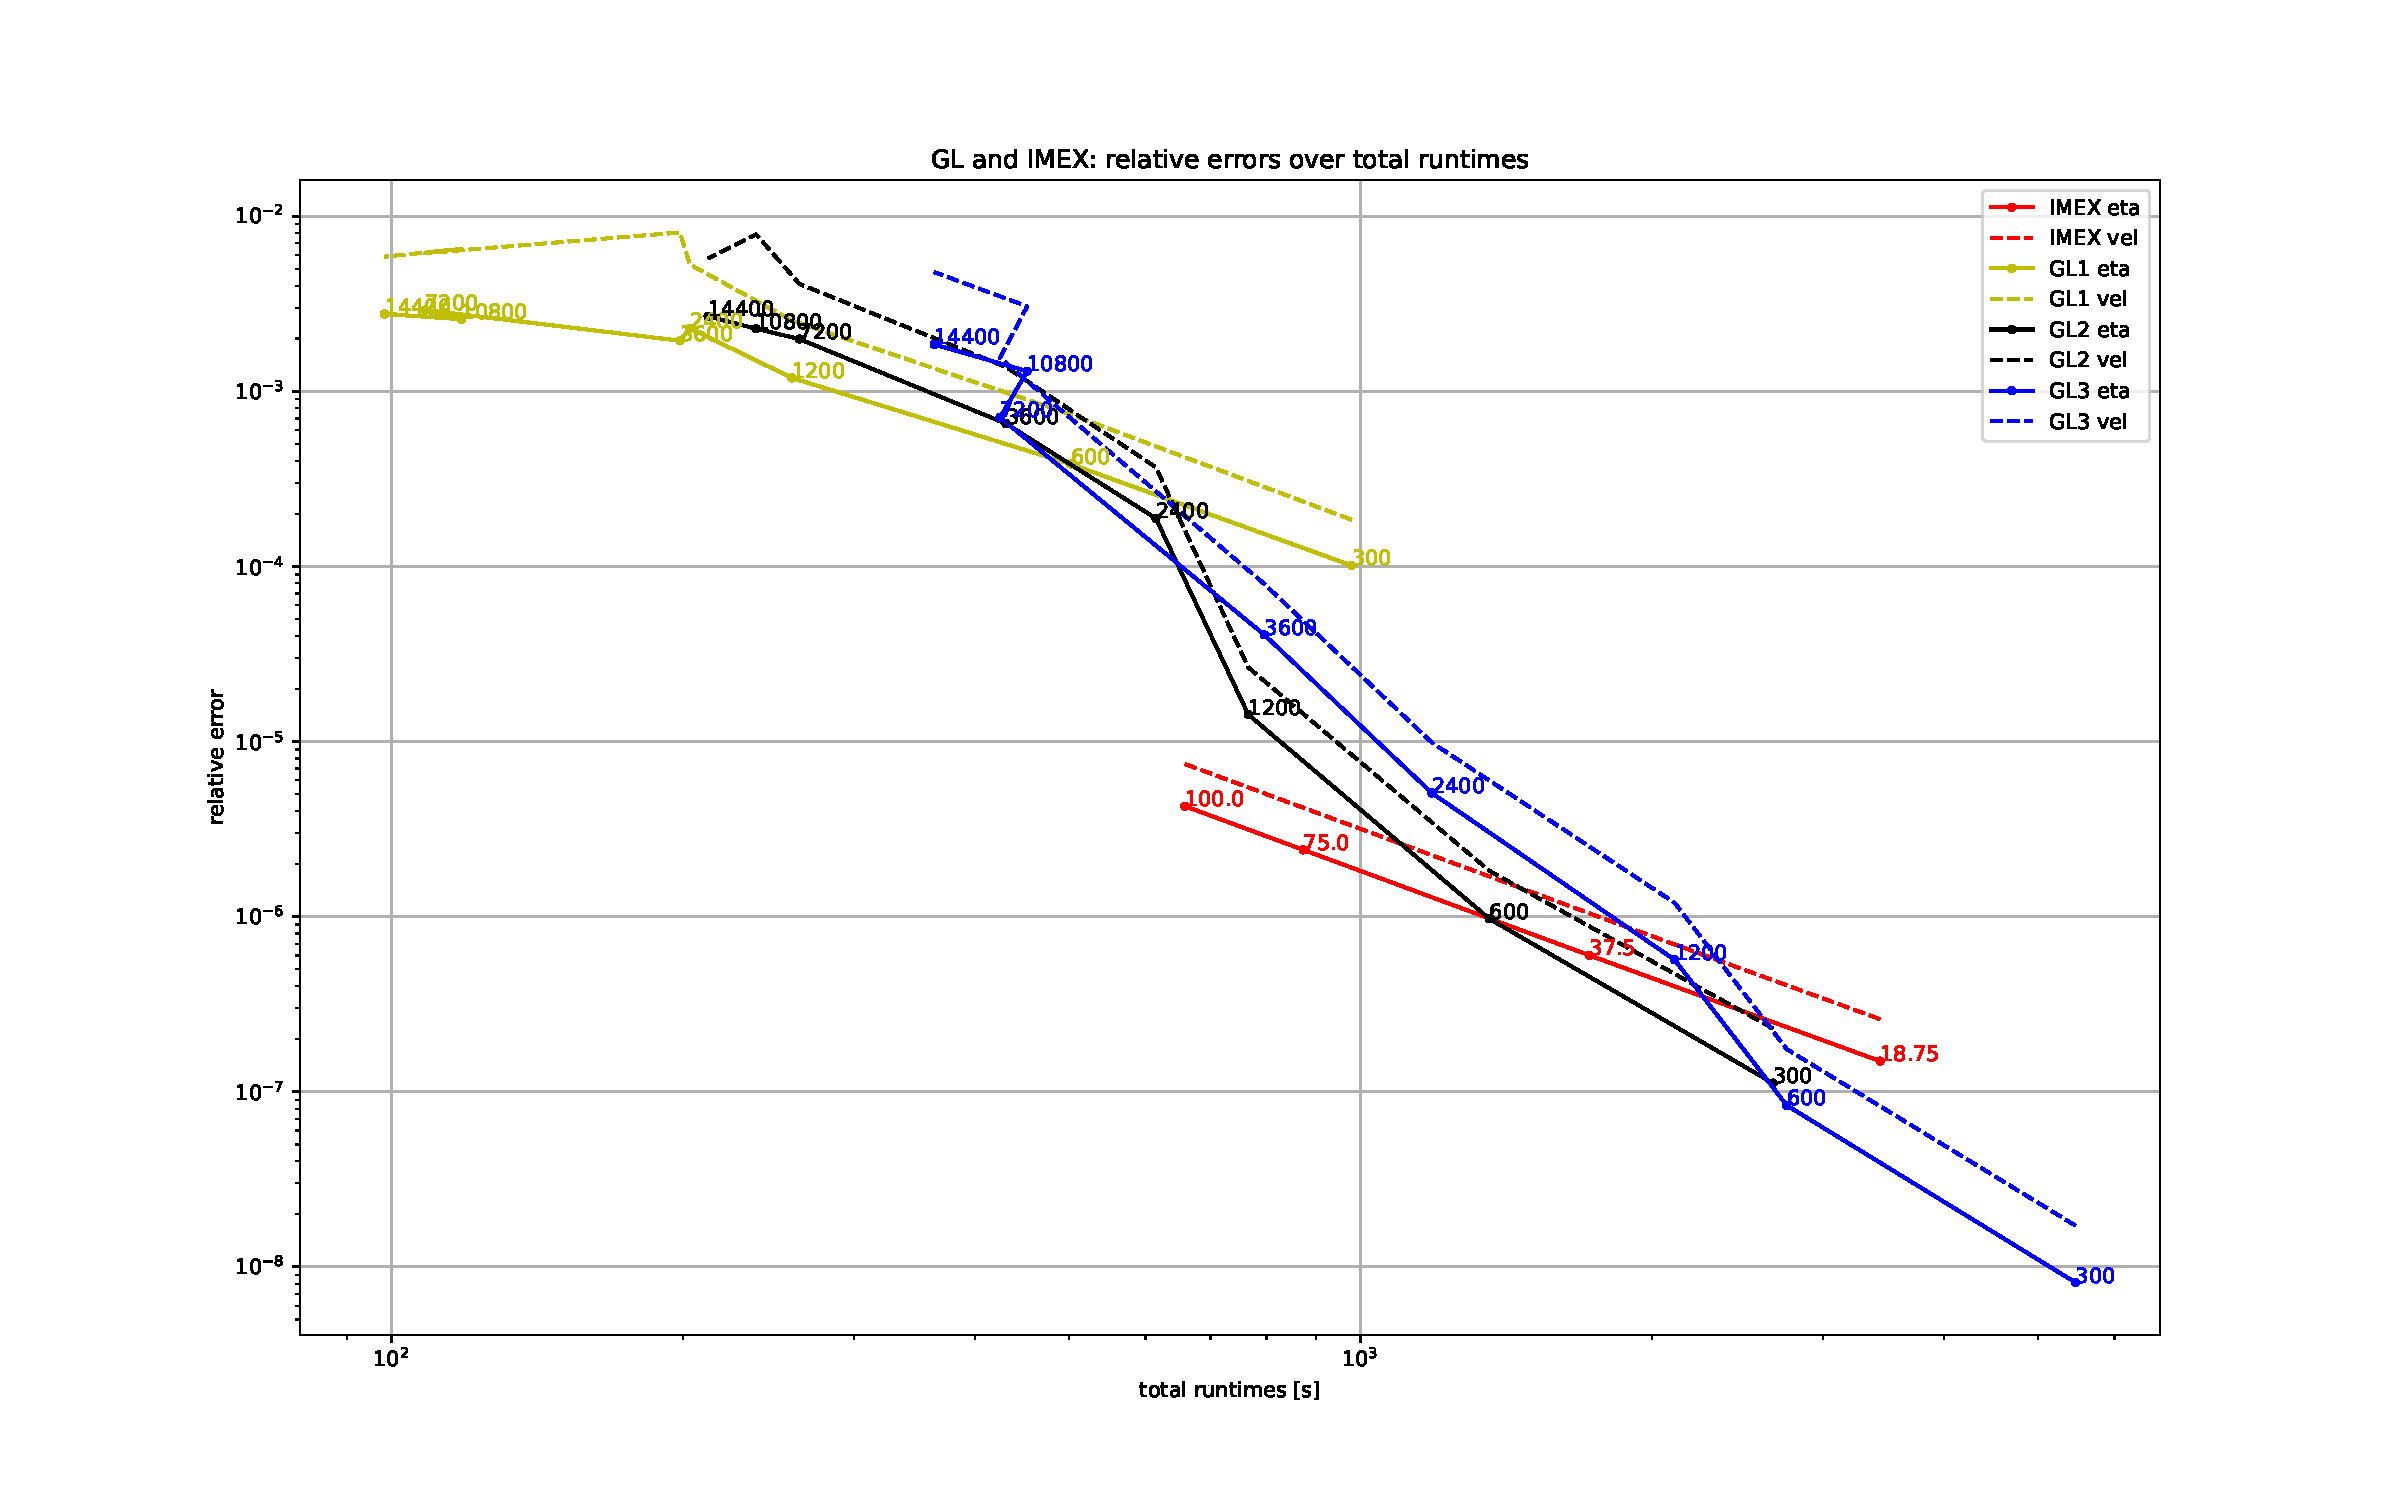
\includegraphics[scale=0.42]{Images/gl_imex.pdf}
\end{tabular}
 \caption{Relative errors of Gauss-Legendre and Imex methods vs total simulation run-times. The numbers on the curves indicate the time step sizes $dt$ used for the corresponding simulation. Solid lines indicate values for the depth field $\eta$ and dashed lines for the velocity fields $ u$.
  }
 \label{err_vs_runtime_gl_imex}
\end{figure}

\begin{figure}[h]\centering
\begin{tabular}{c}
 \hspace{-0.0em}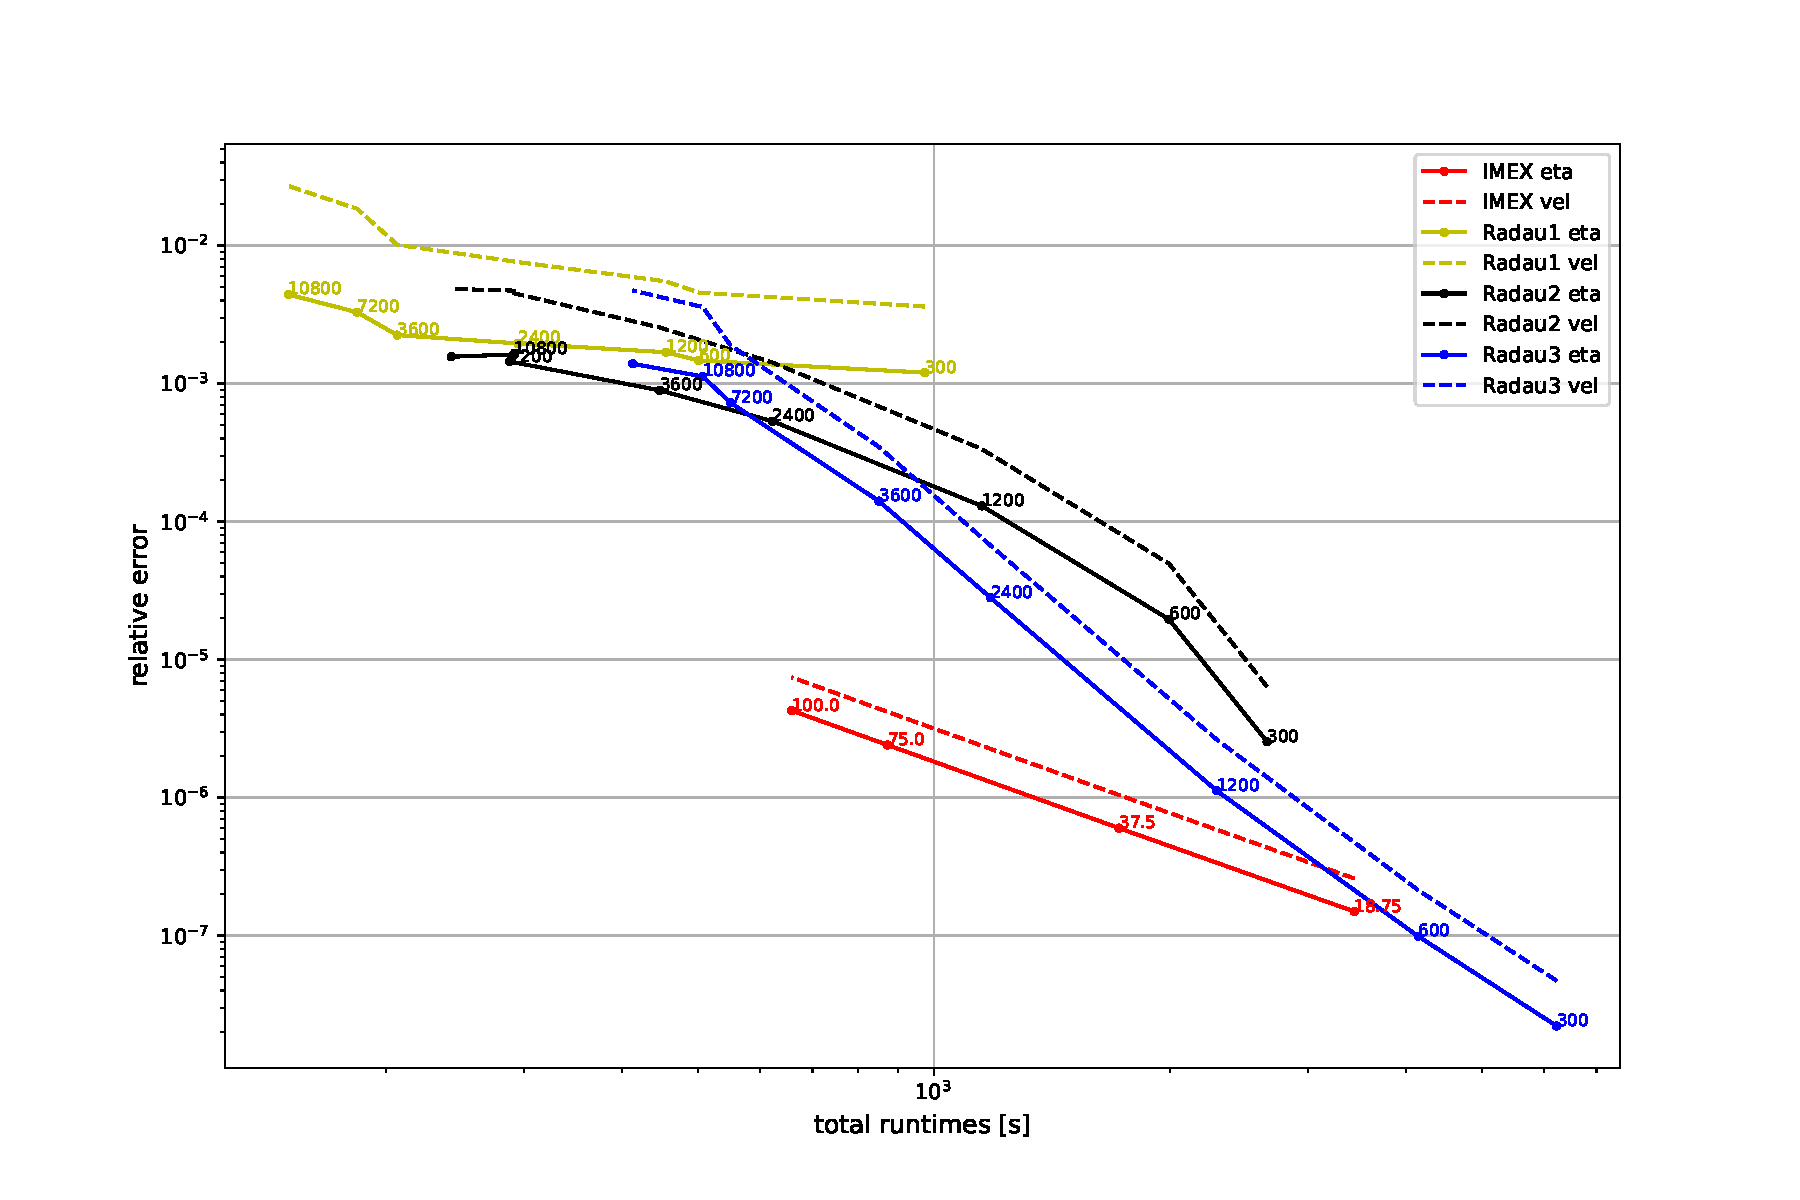
\includegraphics[scale=0.42]{Images/rd_imex.pdf}
\end{tabular}
 \caption{Relative errors of Radau2 and Imex methods vs total simulation run-times. The numbers on the curves indicate the time step sizes $dt$ used for the corresponding simulation. Solid lines indicate values for the depth field $\eta$ and dashed lines for the velocity fields $ u$.
  }
 \label{err_vs_runtime_rd_imex}
\end{figure}


\begin{table}[h]\centering
\begin{tabular}{c|c|c|c|c}
dt    & ref-level &  time    & err-eta      &    err-vel \\ \hline
18.75 & 6         &  3437.80 & 1.494801e-07 &  2.594803e-07 \\
37.50     &     6  &  1722.50 & 6.010706e-07  &1.044124e-06 \\
75.00   &       6  &   873.01 & 2.404467e-06 & 4.181827e-06 \\
100.00     &     6  &   658.81 & 4.271615e-06 & 7.436415e-06
\end{tabular}
\caption{Numerical values for the IMEX simulations.}
\end{table}




\begin{table}[h]\centering
\begin{tabular}{c|c|c|c|c|c}
dt    & ref-level & rk-stages & time  &    err-eta      &    err-vel \\ \hline
300    &       6  &  1    &978.850  &  0.000101 &  0.000185 \\
600    &       6  & 1    &501.970  & 0.000384 &  0.000739\\
1200   &        6 &  1    &258.890 &  0.001193 &  0.002536\\
2400    &       6 &  1    &203.150 &  0.002290 &  0.005305\\
3600   &        6 &  1    &198.420 &  0.001944 &  0.008068\\
7200    &       6  & 1    &108.260 &  0.002910 &  0.006148\\
10800    &       6 & 1    & 118.050 &  0.002580 &  0.006506\\
14400    &       6  & 1    & 98.331 &  0.002766 &  0.005868\\
\end{tabular}
\caption{Numerical values for the Gauss Legendre rk-stages 1 simulations.}
\end{table}








\begin{table}[h]\centering
\begin{tabular}{c|c|c|c|c|c}
dt    & ref-level &  rk-stages & time    & err-eta      &    err-vel \\ \hline
300    &      6    &      2 & 2665.00 & 1.119265e-07 & 2.295523e-07 \\
600    &      6   &       2 & 1357.90 & 9.724745e-07 & 1.827295e-06\\
1200   &       6   &       2  & 765.88 & 1.424818e-05 & 2.644705e-05\\
2400    &      6   &       2 &  614.82 & 1.881205e-04 & 3.679311e-04\\
3600    &      6   &       2 &  430.65 & 6.534951e-04 & 1.375421e-03\\
7200    &      6    &      2  & 263.50 & 1.988320e-03 & 4.106426e-03\\
10800    &      6   &       2 &  237.78 & 2.275762e-03 & 7.882027e-03\\
14400    &      6   &       2 &  212.17 & 2.679312e-03 & 5.744365e-03\\
\end{tabular}
\caption{Numerical values for the Gauss Legendre rk-stages 2 simulations.}
\end{table}





\begin{table}[h]\centering
\begin{tabular}{c|c|c|c|c|c}
dt    & ref-level &  rk-stages & time    & err-eta      &    err-vel \\ \hline
300    &       6   &        3  & 5468.80  & 8.134017e-09  & 1.719576e-08 \\
600     &      6    &       3  & 2752.70  & 8.364238e-08  & 1.753401e-07\\
1200     &      6    &       3  & 2109.30  & 5.666891e-07  & 1.199175e-06\\
2400     &      6    &       3  & 1184.60  & 5.082739e-06  & 9.872072e-06\\
3600      &     6     &      3  &  795.64  & 4.065958e-05  & 7.928632e-05\\
7200      &     6      &     3   & 424.55  & 7.089932e-04  & 1.551004e-03\\
10800     &      6     &      3  &  452.88  & 1.301794e-03  & 3.055263e-03\\
14400      &     6     &      3   & 363.06   &1.851840e-03  & 4.796533e-03\\
\end{tabular}
\caption{Numerical values for the Gauss Legendre rk-stages 3 simulations.}
\end{table}




\begin{table}[h]\centering
\begin{tabular}{c|c|c|c|c|c}
dt    & ref-level &  rk-stages & time    & err-eta      &    err-vel \\ \hline
300    &      6   &       1 & 973.78 & 0.001200 & 0.003610 \\
600    &      6   &       1 & 501.30 & 0.001468 & 0.004560\\
1200   &       6   &       1 & 455.43 & 0.001685 & 0.005498\\
2400   &       6   &       1 & 294.77 & 0.001952 & 0.007593\\
3600    &      6    &      1 & 206.78 & 0.002244 & 0.010134\\
7200   &       6    &      1 & 183.77 & 0.003285 & 0.018488\\
10800   &       6   &       1 & 150.23 & 0.004418 & 0.026992\\
14400   &       6   &       1 &-666.00 & nan & nan
\end{tabular}
\caption{Numerical values for the Radau2 rk-stages 1 simulations.
Note that the time -666 indicates a blow up of the run, hence not error values can be computed.}
\end{table}




\begin{table}[h]\centering
\begin{tabular}{c|c|c|c|c|c}
dt    & ref-level &  rk-stages & time    & err-eta      &    err-vel \\ \hline
300   &        6   &        2 &  2661.20 &  0.000003 &  0.000006\\
600    &       6   &        2 &  1995.20 &  0.000020 &  0.000049\\
1200  &         6   &        2 &  1151.00 &  0.000130 &  0.000336\\
2400   &        6   &        2 &   622.44 &  0.000533 &  0.001421\\
3600   &        6   &        2 &   447.14 &  0.000893 &  0.002546\\
7200    &       6   &        2 &   287.81 &  0.001444 &  0.004587\\
10800   &        6  &         2 &   291.70 &  0.001627 &  0.004711\\
14400    &       6  &         2 &   242.43 &  0.001564 &  0.004848\\
\end{tabular}
\caption{Numerical values for the Radau2 rk-stages 2 simulations.}
\end{table}



\begin{table}[h]\centering
\begin{tabular}{c|c|c|c|c|c}
dt    & ref-level &  rk-stages & time    & err-eta      &    err-vel \\ \hline
300    &       6   &        3  & 6227.40 &  2.214081e-08 &  4.711117e-08\\
600    &       6   &        3 &  4147.20 &  9.890813e-08 &  2.136634e-07\\
1200    &       6  &         3&   2295.40 &  1.120790e-06 &  2.632214e-06\\
2400    &       6  &         3 &  1181.60 &  2.802082e-05 &  6.698549e-05\\
3600    &       6  &         3 &   851.04 &  1.406876e-04 &  3.477579e-04\\
7200    &       6  &         3  &  550.43 &  7.251949e-04 &  1.890284e-03\\
10800   &        6  &         3 &   507.18 &  1.125798e-03 &  3.585997e-03\\
14400     &      6  &         3 &   413.00 &  1.390544e-03 &  4.723006e-03\\
\end{tabular}
\caption{Numerical values for the Radau2 rk-stages 3 simulations.}
\end{table}





\cleardoublepage



\subsection{Dependency of runtimes on number of used CPU cores}


So far, we used for all simulations the same amount of cores, i.e. 16 (no hyperthreading). To have a better understanding of the impact of HPC architectures on our result we next study the impact of using different numbers of cores on the total runtimes.

Table~\ref{tab_imex_cores} shows the dependency of the total runtimes for the above studied Williamson test case 6 for 1 day simulation on mesh level 6. The total runtime, shown in the second column for 16 cores, in the third for 8 cores, and in the fourth for 4 cores depend on the time step size $dt$. The last two columns illustrate the speedup, in all cases of about 1.4 when doubling the number of cores from 8 to 16, and about 1.65 when doubling from 4 to 8 cores.

\begin{table}[h]\centering
\begin{tabular}{c|c|c|c|c|c|c}
dt &  time16  &  time8  & time4  &   16vs8   &   8vs4     & 16vs4     \\\hline
18.75 & 3437.80 & 4953.10 & 8323.2 & 1.440776 & 1.680402  & 2.421083\\
37.50 & 1722.50 & 2475.70 & 4192.0 & 1.437271 & 1.693258  & 2.433672\\
75.00  & 873.01 & 1251.10  &2086.8 & 1.433088 & 1.667972  & 2.390351\\
100.00 &  658.81 &  944.24&  1585.6 & 1.433251 & 1.67923 4& 2.406764
\end{tabular}
\caption{Total runtime of IMEX simulations when using 16, 8 or 4 CPU cores in dependency of the used time step size. The 5th column shows speed up when using 16 rather than 8 cores while the last columns shows such speed up when using 8 rather then 4 cores.}
\label{tab_imex_cores}
\end{table}

Similarly, Table~\ref{tab_irksgl1_cores} illustrates the speedup of the
Irksome GaussLegendre order 1 simulations when using different numbers of
cores for various time step sizes.Here, the speedup when doubling the numbers of cores is about 1.45 in average when doubling the number of cores from 8 to 16, and about 1.65 when doubling from 4 to 8 cores, hence quite similar to the imex scheme. Note that for smaller dt, the speedup is slightly bigger, but it decreases with larger time step sizes.


Tables~\ref{tab_irksgl2_cores} and \ref{tab_irksgl3_cores} show the same information but for Gauss-Legendre 2 and Gauss-Legendre 3, respectively. Given the increasing numbers of DOF for higher order methods, the total runtimes increase here, but we realize that the speedup for the higher order versions are comparable to GL1, although a tiny bit higher then for less Dofs indicating that the HO version seem to better benefit from more CPU cores.


\begin{table}[h]\centering
\begin{tabular}{c|c|c|c|c|c|c}
dt &  time16  &  time8  & time4  &   16vs8       &   8vs4   & 16vs4 \\\hline
 300 & 978.850 & 1479.10 & 2485.40 & 1.511059    & 1.680346 & 2.539102\\
    600 & 501.970  & 746.76 & 1264.30 & 1.487659 & 1.693047 & 2.518676\\
   1200 & 258.890  & 386.97  & 644.79 & 1.494727 & 1.666253 & 2.490594\\
   2400 & 203.150  & 299.47  & 491.16 & 1.474132 & 1.640098 & 2.417721\\
   3600 & 198.420 &  289.11 &  472.88 & 1.457061 & 1.635640 & 2.383227\\
   7200 & 108.260  & 158.95  & 249.78 & 1.468225 & 1.571438 & 2.307223\\
  10800 & 118.050 &  168.39  & 273.80 & 1.426429 & 1.625987 & 2.319356\\
  14400 &  98.331 &  137.50 &  219.78 & 1.398338 & 1.598400 & 2.235104\\
\end{tabular}
\caption{Total runtime of GaussLegendre 1 simulations when using 16, 8 or 4 CPU cores in dependency of the used time step size. The 5th column shows speed up when using 16 rather than 8 cores while the last columns shows such speed up when using 8 rather then 4 cores.}
\label{tab_irksgl1_cores}
\end{table}




\begin{table}[h]\centering
\begin{tabular}{c|c|c|c|c|c|c}
dt &  time16  &  time8  & time4  &   16vs8   &   8vs4  & 16vs4    \\\hline
     300  & 2665.00  & 4158.80  & 7192.90  & 1.560525  & 1.729561 & 2.699024\\
     600  & 1357.90  & 2112.60  & 3621.10  & 1.555785  & 1.714049  & 2.666691 \\
    1200  &  765.88  & 1177.30  & 2065.20  & 1.537186  & 1.754183  & 2.696506\\
    2400  &  614.82   & 903.21  & 1537.40  & 1.469064  & 1.702151  & 2.500569\\
   3600   & 430.65   & 644.89   &1086.70  & 1.497481  & 1.685094  & 2.523395\\
   7200  &  263.50   & 384.85   & 649.56   &1.460531  & 1.687826  & 2.465123\\
  10800   & 237.78   & 347.62   & 557.78  & 1.461940  & 1.604568  & 2.345782 \\
  14400   & 212.17   & 312.52   & 508.26  & 1.472970  & 1.626328  & 2.395532
\end{tabular}
\caption{Total runtime of GaussLegendre 2 simulations when using 16, 8 or 4 CPU cores in dependency of the used time step size. The 5th column shows speed up when using 16 rather than 8 cores while the last columns shows such speed up when using 8 rather then 4 cores.}
\label{tab_irksgl2_cores}
\end{table}




\begin{table}[h]\centering
\begin{tabular}{c|c|c|c|c|c|c }
dt &  time16  &  time8  & time4  &   16vs8   &   8vs4                 & 16vs4 \\\hline
    300  &  5468.80  &  8759.00  &  15414.0  &  1.601631  &  1.759790  &  2.818534\\
    600  &  2752.70  &  4403.80   &  7693.1  &  1.599811  &  1.746923  & 2.794747 \\
   1200  &  2109.30  &  3337.00   &  5775.2  &  1.582041  &  1.730656  & 2.737970 \\
   2400  &  1184.60  &  1846.70   &  3203.8  &  1.558923  &  1.734878  &  2.704542\\
   3600  &   795.64  &  1244.30   &  2150.0  &  1.563898  &  1.727879  &  2.702227\\
   7200   &  424.55   &  647.44   &  1124.2  &  1.525003  &  1.736377  &  2.647980\\
  10800   &  452.88   &  691.13   &  1157.9  &  1.526078  &  1.675372  &  2.556748\\
  14400   &  363.06   &  573.04    &  929.3   & 1.578362   & 1.621702  &  2.559632
\end{tabular}
\caption{Total runtime of GaussLegendre 3 simulations when using 16, 8 or 4 CPU cores in dependency of the used time step size. The 5th column shows speed up when using 16 rather than 8 cores while the last columns shows such speed up when using 8 rather then 4 cores.}
\label{tab_irksgl3_cores}
\end{table}



Finally, in Table~\ref{tab_irksrd123_cores} we show only speedups for the Radau 1 (RD1),
Radau 2 (RD2) and Radau 3 RD3) methods when doubling the number of course (similarly to above).
See see that the speedup rates are comparable to the ones obtained for any of the GaussLegendre methods.

\begin{table}[h]\centering
\begin{scriptsize}
\begin{tabular}{c|c|c|c||c|c|c||c|c|c}
 dt & RD1 16vs8   & RD1  8vs4  & RD1 16vs4 & RD2 16vs8   & RD2  8vs4 & RD2 16vs4 &   RD3 16vs8
 & RD3  8vs4  & RD3 16vs4\\ \hline
   300  &   1.539362 & 1.654903 &2.547495 &  1.559409 & 1.734572 & 2.704908 & 1.584337 &  1.746450  & 2.766965\\
   600  &   1.489607 & 1.688540 & 2.515260& 1.537340 & 1.713950 & 2.634924 &   1.586299 & 1.745938  &2.769579 \\
  1200  &   1.477944 & 1.664983 & 2.460751& 1.530582 & 1.709031 & 2.615812 & 1.573103 & 1.737185 &2.732770 \\
  2400  &  1.468772 & 1.645109  & 2.416291& 1.520339 & 1.694670 & 2.576473 & 1.567282 & 1.733409 & 2.716740\\
  3600  &  1.452123 & 1.638958  & 2.379969& 1.489243 & 1.691695 & 2.519345 & 1.565379 & 1.727143 & 2.703633\\
  7200  & 1.408500 & 1.614395-  & 2.273875&  1.489768&  1.652774 & 2.462249 & 1.591538 & 1.650058 & 2.626129\\
 10800 &   1.396592 & 1.819265  & 2.540771& 1.452383 & 1.653543 & 2.401577 & 1.540597 & 1.619612 &2.495169 \\
 14400 &  NaN      &  1.259854 & NaN & 1.472219 & 1.619568 & 2.384358 &  1.570823 & 1.619422  &2.543826
\end{tabular}
\caption{Total runtime of Radau 1,2,3 simulations when using 16, 8 or 4 CPU cores in dependency of the used time step size.
\checkit{The 2nd, 4th, 6th column shows speed up when using 16 rather than 4 cores while the 3rd, 5th, 7th columns shows such speed up when using 8 rather then 4 cores. RD1 is Radau 1, RD2 is Radau 2, and RD3 is Radau 3. NaN in the table indicates that for the given time step size and method, the solver did not converge, hence there is not total runtime available (here for Radau 3 with dt of 14400).}}
\label{tab_irksrd123_cores}
\end{scriptsize}
\end{table}


\cleardoublepage

\subsection{Iteration counts tables}

\begin{table}[h]\centering
\begin{scriptsize}
 \begin{tabular}{c||c|c|c||c|c|c||c|c|c}
   dt & rk-stages  &  its-per-steps  &   niter  &  rk-stages  &  its-per-steps  &   niter  &  rk-stages  &  its-per-steps  &   niter\\ \hline
  300  &          1    &     4.000000  &  1152.0    &    2   &    4.000000  &  1152.0   &      3   &      4.000000  &  1152.0 \\
   600  &         1     &    4.000000  &   576.0    &    2    &   4.055556  &   584.0    &     3    &     4.000000   &  576.0 \\
  1200   &         1   &      4.000000   &  288.0   &    2   &      4.722222  &   340.0    &        3    &     6.833333  &   492.0\\
  2400    &        1    &     7.250000   &  261.0   &    2   &       8.194444   &  295.0    &        3    &     8.000000   &  288.0\\
  3600     &       1    &    11.708333  &   281.0   &    2   &    8.958333   &  215.0     &       3    &     8.000000  &   192.0 \\
  7200     &       1   &     11.916667  &   143.0    &   2   &     11.416667  &   137.0    &        3   &      8.500000  &   102.0\\
  10800    &        1   &     22.375000 &    179.0   &   2   &     16.750000   &  134.0    &        3     &   16.250000   &  130.0 \\
  14400    &        1   &     24.166667  &   145.0   &   2   &     20.500000   &  123.0     &       3     &   17.666667   &  106.0
\end{tabular}
\caption{Iteration per step (its-per-step) and total iteration count (niter) vs $dt$ for the Gauss-Legendre 1, 2, 3 methods.}
\label{tab_niter_vs_dt}
\end{scriptsize}
\end{table}


\begin{table}[h]\centering
\begin{scriptsize}
\begin{tabular}{c||c|c|c||c|c|c||c|c|c}
 dt & rk-stages  &  its-per-steps  &   niter  &  rk-stages  &  its-per-steps  &   niter  &  rk-stages  &  its-per-steps  &   niter\\ \hline
300  &        1 &      4.000000 & 1152.0 &         2 &      4.000000 & 1152.0 &         3&       5.000000 & 1440.0\\
600  &        1  &     4.000000 &  576.0 &         2  &     6.777778 &  976.0  &        3 &      6.770833 &  975.0\\
1200  &        1  &     8.750000&   630.0 &         2  &     8.000000 &  576.0  &        3 &      7.736111 &  557.0\\
2400   &       1   &   12.027778 &  433.0  &        2   &    8.777778 &  316.0   &       3  &     8.000000  & 288.0\\
3600    &      1    &  12.250000 &  294.0   &       2    &   9.500000 &  228.0    &      3   &    9.000000  & 216.0\\
7200     &     1   &   24.333333  & 292.0    &      2     & 13.083333 &  157.0     &     3    &  12.166667  & 146.0\\
10800     &     1   &   30.375000 &  243.0    &      2  &    21.875000 &  175.0     &     3    &  19.000000 &  152.0\\
14400      &    1   & -666.000000 & -3996.0    &      2 &     24.333333 &  146.0     &     3    &  20.833333 &  125.0
\end{tabular}
\caption{Iteration per step (its-per-step) and total iteration count (niter) vs $dt$ for the RADAUII2 1,2,3 methods.
\checkit{Substitute -666 by a star and mention that there is no result because the simulation crashed for these values}}
\label{tab1_niter_vs_dt}
\end{scriptsize}
\end{table}







% \multirow{3}{*}{} & \multicolumn{2}{c|}{User B} & \multirow{3}{*}{X} & %
%     \multicolumn{2}{c|}{User C} & \multirow{3}{*}{D}\\


\begin{table}[h]\centering
\begin{scriptsize}
\begin{tabular}{c|c|c|c|c|c|c|c|c|c}
\multicolumn{0}{c|}{dt} &
\multicolumn{2}{c|}{300} &
\multicolumn{2}{c|}{600} &
\multicolumn{2}{c|}{1200} &
\multicolumn{2}{c|}{2400}
\\ \hline\hline
ref-level &   its per step &   niter & its per step &   niter & its per step &   niter & its per step &   niter\\ \hline
     3    &      4.000000  & 1152.0 & 4.000000 & 576.0 & 4.0 & 288.0 & 4.00 & 144.0\\
     4   &      4.000000  & 1152.0  & 4.006944 & 577.0 & 4.0 & 288.0 & 4.00 & 144.0\\
     5   &      4.017361  & 1157.0  & 4.000000 & 576.0 & 4.0 & 288.0 & 4.00 & 144.0\\
     6   &      4.000000  & 1152.0 & 4.000000 & 576.0  & 4.0 & 288.0 & 7.25 & 261.0\\
%     ref_level   dt  its per step  niter
% 22          3  600      4.000000  576.0
% 21          4  600      4.006944  577.0
% 23          5  600      4.000000  576.0
% 20          6  600      4.000000  576.0
%     ref_level    dt  its per step  niter
% 32          3  1200           4.0  288.0
% 28          4  1200           4.0  288.0
% 29          5  1200           4.0  288.0
% 35          6  1200           4.0  288.0
%     ref_level    dt  its per step  niter
% 36          3  2400          4.00  144.0
% 38          4  2400          4.00  144.0
% 37          5  2400          4.00  144.0
% 46          6  2400          7.25  261.0
\end{tabular}
\bigskip

\begin{tabular}{c|c|c|c|c|c|c|c|c|c}
\multicolumn{0}{c|}{dt} &
\multicolumn{2}{c|}{3600} &
\multicolumn{2}{c|}{7200} &
\multicolumn{2}{c|}{14400}
\\ \hline\hline
ref-level &   its per step &   niter & its per step &   niter & its per step &   niter  \\ \hline
     3    &   4.000000  & 96.0 & 4.000000 &  48.0&  8.166667 &  49.0\\
     4   &     4.000000 &  96.0 &8.000000 &  96.0 &8.500000  & 51.0\\
     5   &    7.541667 & 181.0 & 10.833333 & 130.0&12.333333 &  74.0 \\
     6   &   11.708333 & 281.0 & 11.916667 & 143.0&  24.166667 & 145.0
%     ref_level    dt  its per step  niter
% 48          3  3600      4.000000   96.0
% 56          4  3600      4.000000   96.0
% 51          5  3600      7.541667  181.0
% 58          6  3600     11.708333  281.0
%     ref_level    dt  its per step  niter
% 64          3  7200      4.000000   48.0
% 66          4  7200      8.000000   96.0
% 69          5  7200     10.833333  130.0
% 70          6  7200     11.916667  143.0
%     ref_level     dt  its per step  niter
% 88          3  14400      8.166667   49.0
% 92          4  14400      8.500000   51.0
% 89          5  14400     12.333333   74.0
% 93          6  14400     24.166667  145.0
\end{tabular}
\caption{GaussLegendre, rk-stages 1}
\label{tab_niter_vs_spatial}
\end{scriptsize}
\end{table}



\begin{table}[h]\centering
\begin{scriptsize}
\begin{tabular}{c|c|c|c|c|c|c|c|c|c}
\multicolumn{0}{c|}{dt} &
\multicolumn{2}{c|}{300} &
\multicolumn{2}{c|}{600} &
\multicolumn{2}{c|}{1200} &
\multicolumn{2}{c|}{2400}
\\ \hline\hline
ref-level &   its per step &   niter & its per step &   niter & its per step &   niter & its per step &   niter\\ \hline
        3 &      4.0  &      1152.0 &            4.0 &   576.0 &       4.000000 &   288.0 &       4.000000 &   144.0\\
        4 &      4.0  &      1152.0 &            4.0 &   576.0 &       4.000000 &   288.0 &       4.000000 &   144.0\\
        5 &      4.0  &      1152.0 &            4.0 &   576.0 &       4.000000 &   288.0 &       6.611111 &   238.0\\
        6 &      4.0  &      1152.0 &            4.0 &   576.0 &       6.833333 &   492.0 &       8.000000 &   288.0
\end{tabular}
\bigskip

\begin{tabular}{c|c|c|c|c|c|c|c|c|c}
\multicolumn{0}{c|}{dt} &
\multicolumn{2}{c|}{3600} &
\multicolumn{2}{c|}{7200} &
\multicolumn{2}{c|}{14400}
\\ \hline\hline
ref-level &   its per step &   niter & its per step &   niter & its per step &   niter  \\ \hline
       3 &      4.000000  & 96.0 &       7.916667  & 95.0 &    7.333333 &  44.0\\
       4 &      7.208333  & 173.0 &      7.916667  & 95.0 &    8.166667 &  49.0\\
       5 &      8.000000  & 192.0 &      8.000000  & 96.0 &    8.500000 &  51.0\\
       6 &      8.000000  & 192.0 &      8.500000  &102.0 &   17.666667 & 106.0
\end{tabular}
\caption{GaussLegendre, rk-stages 3}
\label{tab_niter_vs_spatial}
\end{scriptsize}
\end{table}


Note: Radau II behaves very similarly with respect to the iteration count: i.e.
its per step increases with dt, but this effect is also less pronounced for higher
order methods (not shown).







%
%
%
%
% \begin{table}[h]\centering
% \color{red}
% \begin{tabular}{c|c|c|c|c|c|c|c}
%  dt & RD1 16vs8   & RD1  8vs4  & RD2 16vs8   & RD2  8vs4   & RD3 16vs8   & RD3  8vs4 \\ \hline
%    300  &   1.539362 & 1.654903 &  1.559409 & 1.734572 & 1.584337 &  1.746450 \\
%    600  &   1.489607 & 1.688540 &  1.537340 & 1.713950 & 1.586299 & 1.745938 \\
%   1200  &   1.477944 & 1.664983 &  1.530582 & 1.709031 & 1.573103 & 1.737185\\
%   2400  &  1.468772 & 1.645109  &  1.520339 & 1.694670 & 1.567282 & 1.733409\\
%   3600  &  1.452123 & 1.638958  &  1.489243 & 1.691695 & 1.565379 & 1.727143\\
%   7200  & 1.408500 & 1.614395-  &   1.489768&  1.652774 & 1.591538 & 1.650058\\
%  10800 &   1.396592 & 1.819265  &  1.452383 & 1.653543 & 1.540597 & 1.619612\\
%  14400 &  NaN      &  1.259854 &   1.472219 & 1.619568 &  1.570823 & 1.619422
% \end{tabular}
% \caption{Total runtime of Radau 1,2,3 simulations when using 16, 8 or 4 CPU cores in dependency of the used time step size.
% The 2nd, 4th, 6th column shows speed up when using 16 rather than 8 cores while the 3rd, 5th, 7th columns shows such speed up when using 8 rather then 4 cores. RD1 is Radau 1, RD2 is Radau 2, and RD3 is Radau 3.}
% \label{tab_irksrd123_cores_old}
% \end{table}











%
%
% \vspace{10em}
%
%
% %  \end{minipage}\hfill
% % \begin{minipage}{0.55\linewidth}
% \begin{figure}[h]\centering
% \begin{tabular}{cc}
%  \hspace{-0.4em}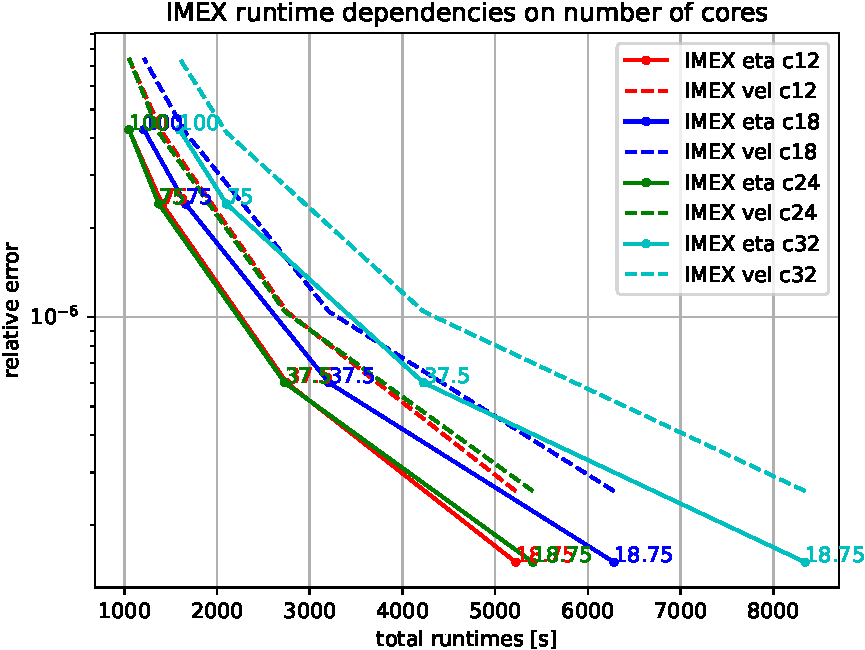
\includegraphics[scale=0.56]{Images/Figure_1_new1-crop.pdf}
%   \hspace{-0.7em}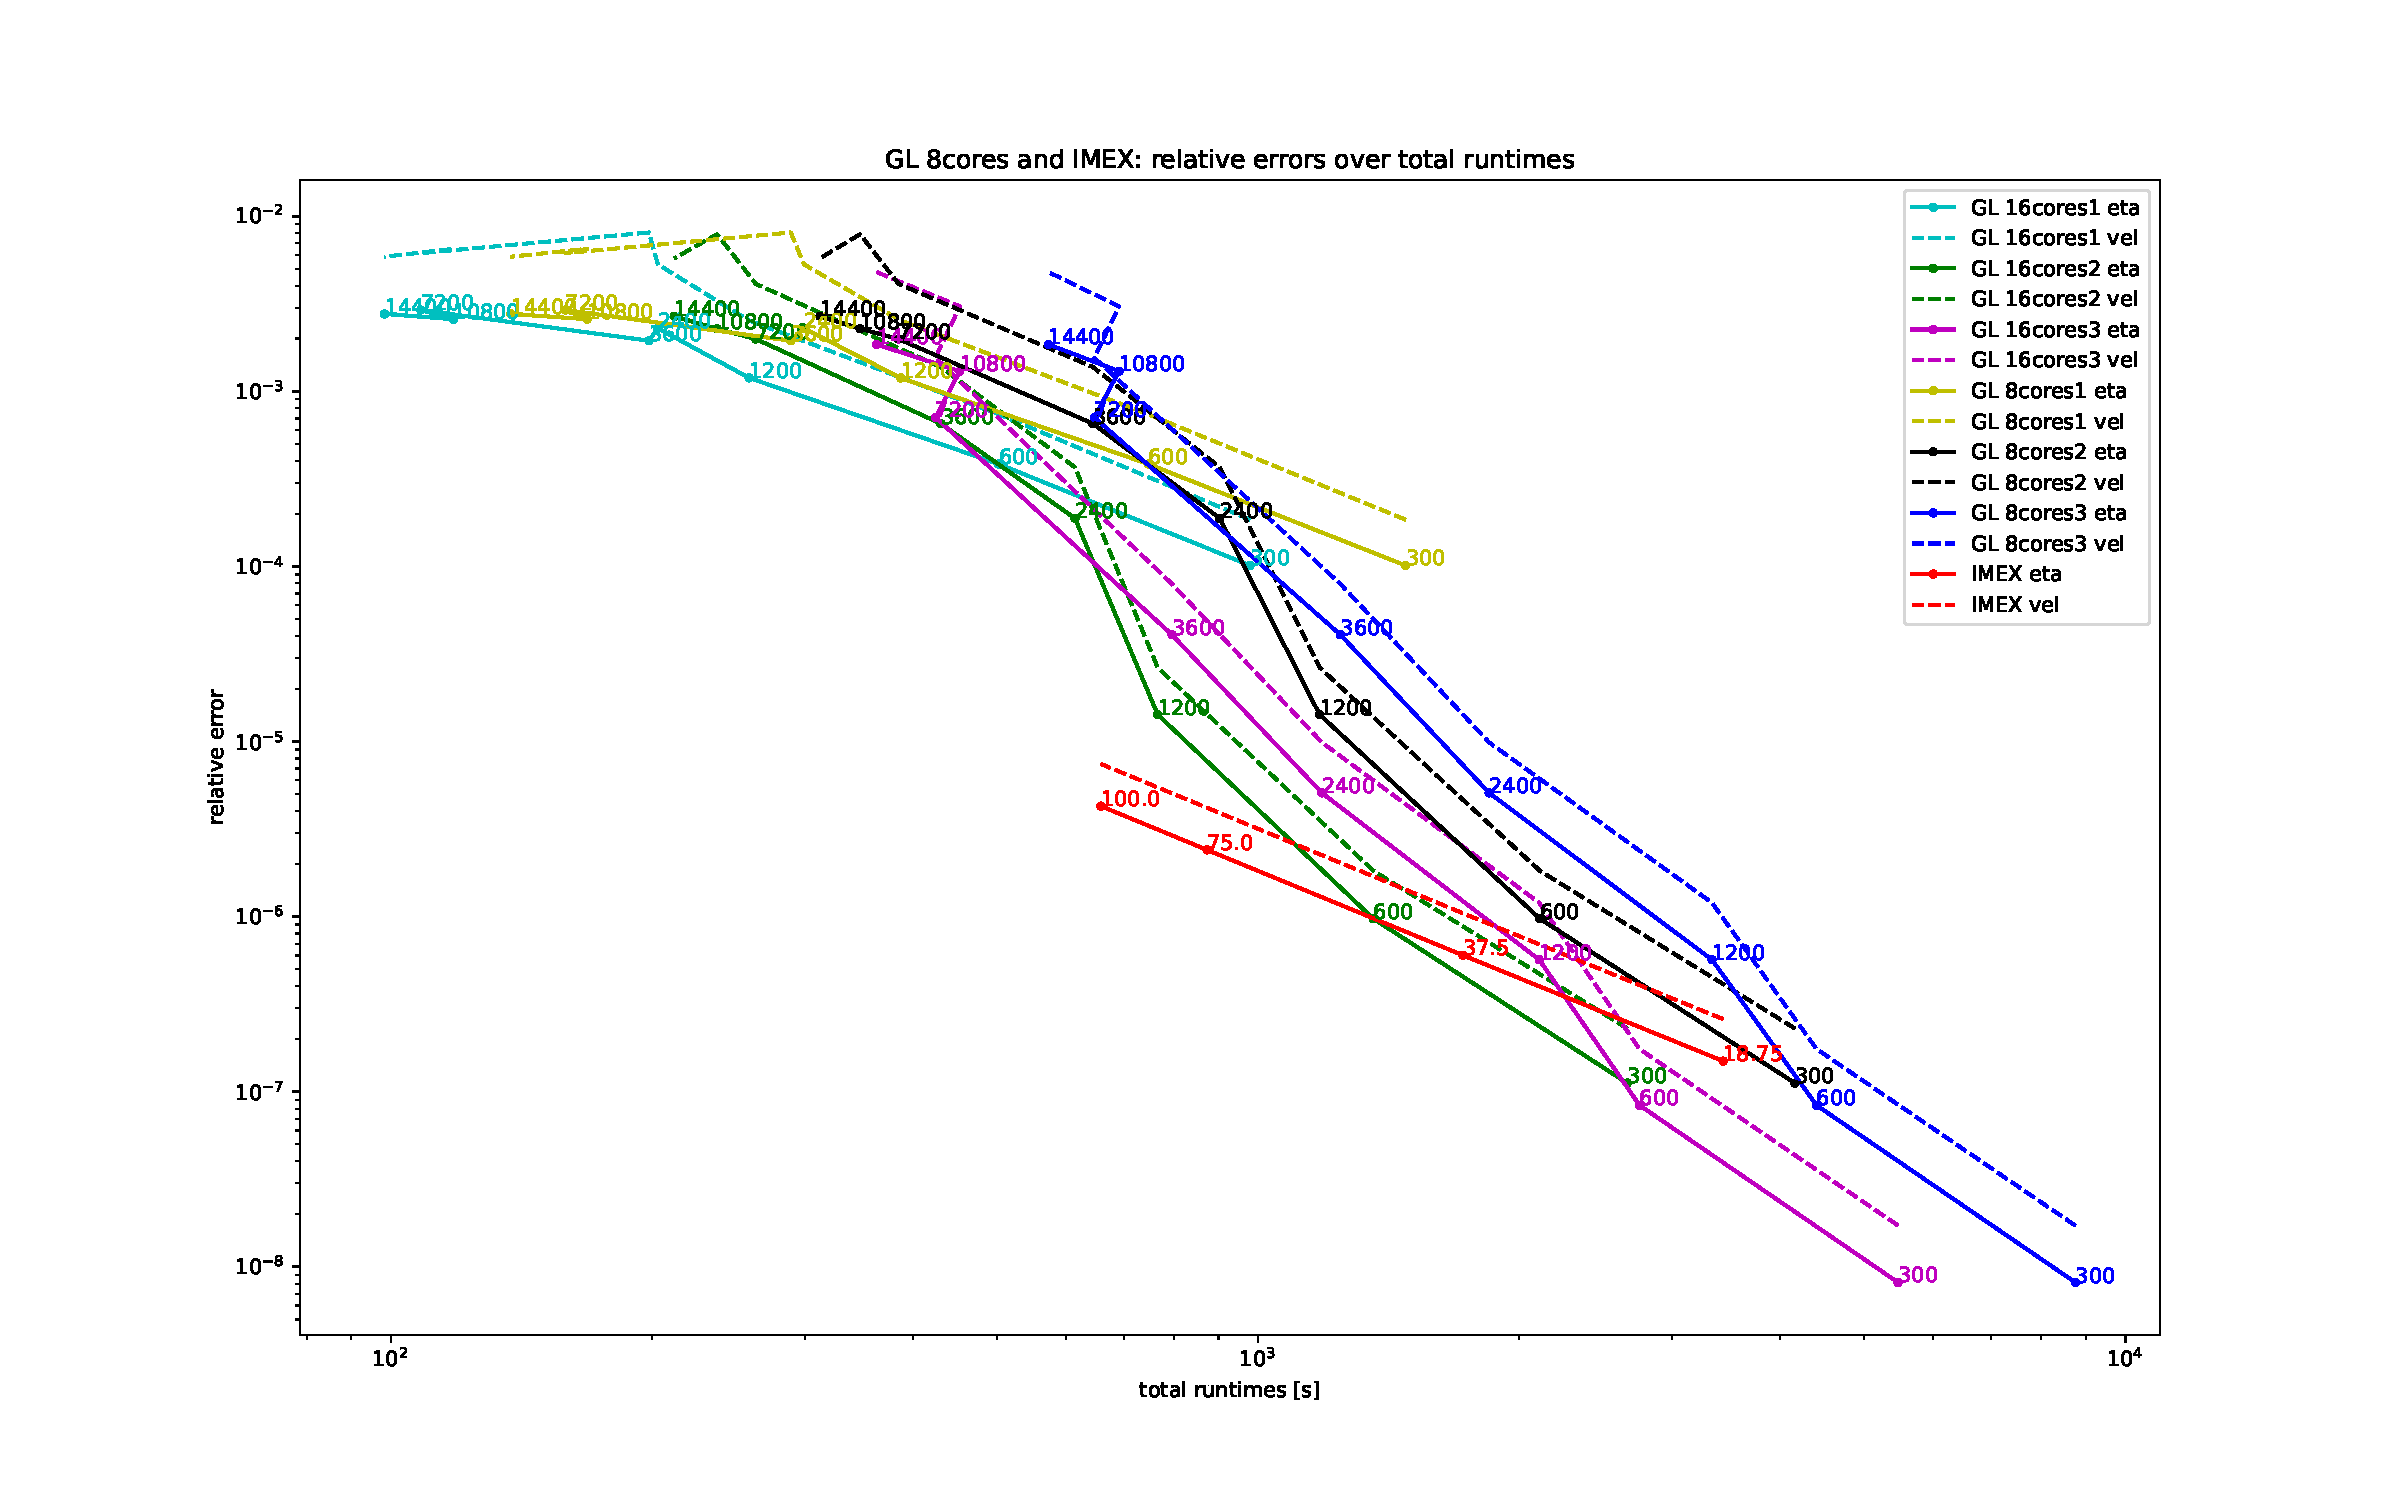
\includegraphics[scale=0.26]{Images/gd_imex_16vs8cores.pdf}
%    \end{tabular}
% \caption{dependency of total runtimes of IMEX scheme (left) and
% IRKs GL scheme (right) on the number of available CPU-cores.
%   }
%   \label{tc6_???}
%   \end{figure}
%  % \end{minipage}



%
%
% \noindent \textcolor{blue}{\textbf{Total runtimes vs. relative errors}}
%
%   Figure 5 summarized the numerical results, i.e. total runtimes vs
%   relative errors of depth $\rho$ and velocity $ u$ fields for ARK2 IMEX
%   scheme, and for Gauss-Legendre (GL) schemes of order 1 (GL1), order 3 (GL2) and order 5 (GL3).
%
%  \begin{figure}[t]\centering
%  \begin{tabular}{cc}
%  \hspace{-0.2em}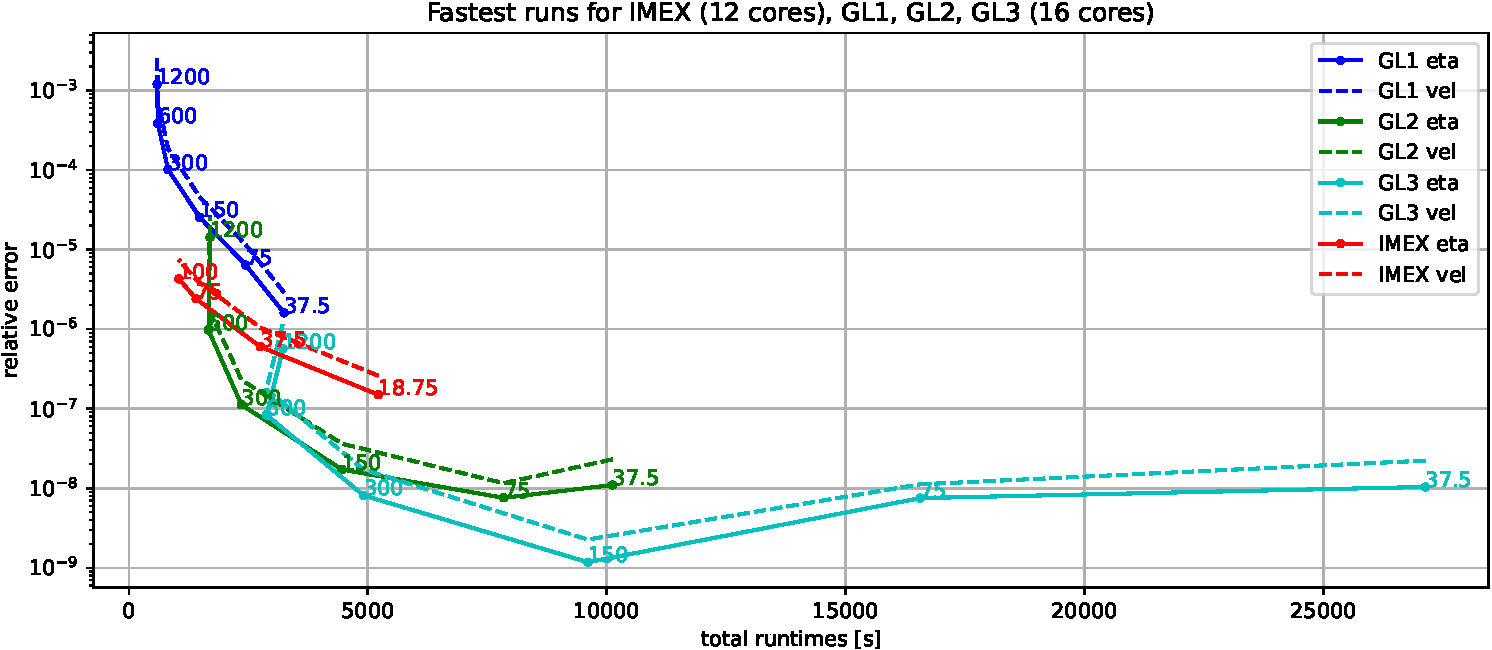
\includegraphics[scale=0.52]{Images/Figure_2_new3-crop.pdf} &
%  %\hspace{-0.95em}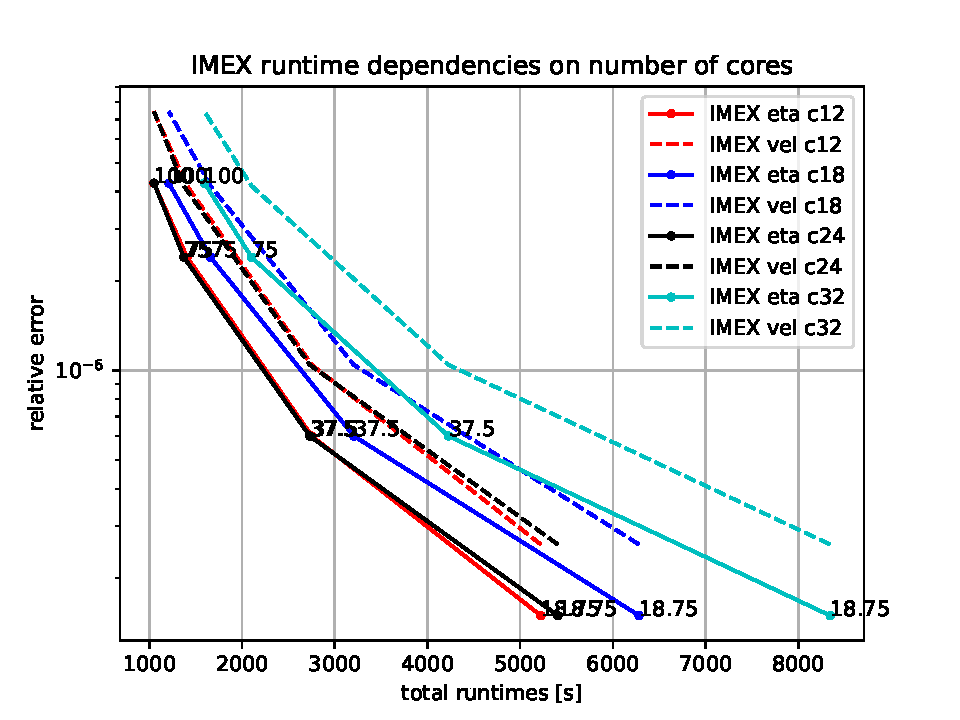
\includegraphics[scale=1.19]{Images/Figure_1_new.pdf}
%   \end{tabular}\vspace{-10pt}
%   \caption*{{\bfseries Figure 5}: relative errors (y-axis)
%   of depth (eta) and velocity (vel) fields against the
%   total runtimes of the simulations depending on the chosen schemes
%   (IMEX, GL1, GL2, GL3). The total runtimes depend on the schemes,
%   the time step sizes (colored figures) and on the number of available CPU-cores
%   (cf. Figure 4).
%
%   }
%   \label{fig2}
%   \end{figure}





 \cleardoublepage


\section{Conclusions}

   \begin{itemize}
    \item Our benchmark tests are \textbf{fair comparisons} between implicit RK schemes (of different orders) from Irksome with the ARK2 IMEX scheme, all using the same monolithic solver in Firedrake.

%    \item Figure 4 shows that under such 'fair' conditions, 3rd-order GL2 is more efficient than 2nd-order ARK2 IMEX: either it is two orders of magnitude more accurate or it requires much less runtime.
   \item Figure 5 shows that under such 'fair' conditions:\\
   (i) 3rd-order GL2 is a little slower than 2nd-order ARK2 IMEX, but about one order of magnitude more accurate; \\
   (ii) 1st order GL1 is slightly quicker but less accurate.

  \item So far, we did not explore advanced solver options, so further speedup for RK methods can be achieved.


   \item Hence, the assumption that IMEX schemes are the fastest schemes for atmosphere/ocean simulation is not necessarily correct.

   \item \textbf{Outlook:} the flexibility of Irksome in easily choosing different accuracy-orders for a vast variety of implicit RK methods allows us to further explore even more efficient time integrators.
   \end{itemize}

\bibliography{refs}

%% \begin{thebibliography}{8}
%% \bibitem{CotterShipton12} Cotter, Colin J., Jemma Shipton. "Mixed finite elements for numerical weather prediction." Journal of Computational Physics 231, no. 21 (2012): 7076-7091.

%% \bibitem{CotterShipton23}
%% \checkit{ADD PAPER DETAILS}

%% \bibitem{Farrell21} Farrell, Patrick E., Robert C. Kirby, Jorge Marchena-Menendez. "Irksome: Automating Runge-Kutta time-stepping for FE methods." ACM Transactions on Math. Software (TOMS) 47, no. 4 (2021): 1-26.

%% \bibitem{Giraldo13} Giraldo, Francis X., James F. Kelly, and Emil M. Constantinescu. "Implicit-explicit formulations of a three-dimensional nonhydrostatic unified model of the atmosphere (NUMA)." SIAM Journal on Scientific Computing 35, no. 5 (2013): B1162-B1194.
%% \end{thebibliography}






\end{document}
